%%%%%%%%%%%%%%%%%%%%%%%%%%%%%%%%%%%%%%%%%%%%%%%%%%%%%%%%%%%%%%%
%
% Welcome to Overleaf --- just edit your LaTeX on the left,
% and we'll compile it for you on the right. If you open the
% 'Share' menu, you can invite other users to edit at the same
% time. See www.overleaf.com/learn for more info. Enjoy!
%
%%%%%%%%%%%%%%%%%%%%%%%%%%%%%%%%%%%%%%%%%%%%%%%%%%%%%%%%%%%%%%%
\documentclass[usenames,dvipsnames]{beamer}

\usepackage{xcolor}
\usepackage{tikz}
\usepackage{hyperref}
\usepackage{ulem}
\usepackage{smartdiagram}
% \usepackage{enumitem}
\usepackage{setspace}
\usepackage{animate}
\usepackage{listings}
\usepackage{minted}

\usetheme{Berkeley}
\usecolortheme{default}
\usepackage{epigraph}

\definecolor{IDEFICSDarkblue}{RGB}{5, 23, 77}
\definecolor{IDEFICSTurquoise}{RGB}{96, 186, 155}
\definecolor{IDEFICSGrey}{RGB}{111, 111, 111}
\definecolor{IDEFICSBlue}{RGB}{9, 30, 84}

\usecolortheme[named=IDEFICSDarkblue]{structure}

\setbeamercolor{example text}{fg=IDEFICSTurquoise}
\setbeamercolor{normal text}{fg=IDEFICSGrey}
\setbeamercolor{section title}{fg=IDEFICSBlue}
\setbeamercolor{logo}{bg=IDEFICSDarkblue}
\setbeamercolor{title}{fg=IDEFICSBlue, bg=white}
\setbeamercolor{subtitle}{fg=IDEFICSBlue}
\setbeamercolor{sidebar}{bg=white}
\setbeamercolor{section in sidebar shaded}{fg=IDEFICSGrey}
\setbeamercolor{subsection in sidebar shaded}{fg=IDEFICSGrey}
\setbeamercolor{section in sidebar}{fg=IDEFICSDarkblue}
\setbeamercolor{subsection in sidebar}{fg=IDEFICSDarkblue}

\setbeamerfont{footline}{size=\small, series=\bfseries}
\setbeamerfont{subsection in sidebar}{size*={4.5pt}{4.1pt}, series=\bfseries}
\setbeamerfont{frametitle}{size=\large, series=\bfseries}
\setbeamerfont{framesubtitle}{size=\large, series=\mdseries}

% customize frametitle to let a right margin for video
\makeatletter
\setbeamertemplate{frametitle}{%
    \nointerlineskip%
    \vskip-\beamer@headheight%
    \vbox to \beamer@headheight{%
      \vfil
      \leftskip=-\beamer@leftmargin%
      \advance\leftskip by0.3cm%
      \rightskip=-\beamer@rightmargin%
      \advance\rightskip by2.3cm plus1fil%  modify right margin
      {\usebeamercolor[fg]{frametitle}
          \usebeamerfont{frametitle}\insertframetitle\par}% 
      {\usebeamercolor[fg]{framesubtitle}
           \usebeamerfont{framesubtitle}\insertframesubtitle\par}%
      \vbox{}%
      \vskip-1em%
      \vfil
    }%
  }
\makeatother


% add a separation line to the sidebar
\makeatletter
\addtobeamertemplate{sidebar left}
  {}
  {\smash{\hspace*{\beamer@sidebarwidth}\textcolor{gray!50}{\rule{0.5pt}{\paperheight}}}}
\makeatother


\hypersetup{
    colorlinks=true,
    linkcolor=IDEFICSBlue,
    filecolor=IDEFICSTurquoise,      
    urlcolor=IDEFICSTurquoise,
    }

\setlength{\epigraphwidth}{0.9\textwidth}


%----------------------------------------------------------------------------
% Title slide configuration
\title[Intro to DL] %optional
{Introduction to Deep Learning}
\subtitle{A practical approach}
% \author[M. Jacquemont] 
\author[Mikaël J.]
{Mikaël Jacquemont}

\institute[LAPP]
{
  Laboratoire d'Annecy de Physique des Particules - IN2P3\\
  Univ. Savoie Mont Blanc, CNRS
}

\date[Escape school 2022]
{ESCAPE Summer School 2022}

\titlegraphic{
    \begin{center}
        
\includegraphics[height=0.5cm]{figures/LogoIDEFICS_SANSbaseline_H_RVB.png}\hspace*{.75cm}~%
        
\includegraphics[height=0.5cm]{figures/logo_cnrs.png}\hspace*{.75cm}~%
        
\includegraphics[height=0.5cm]{figures/Logo_lapp_2020.png}\hspace*{.75cm}~%
        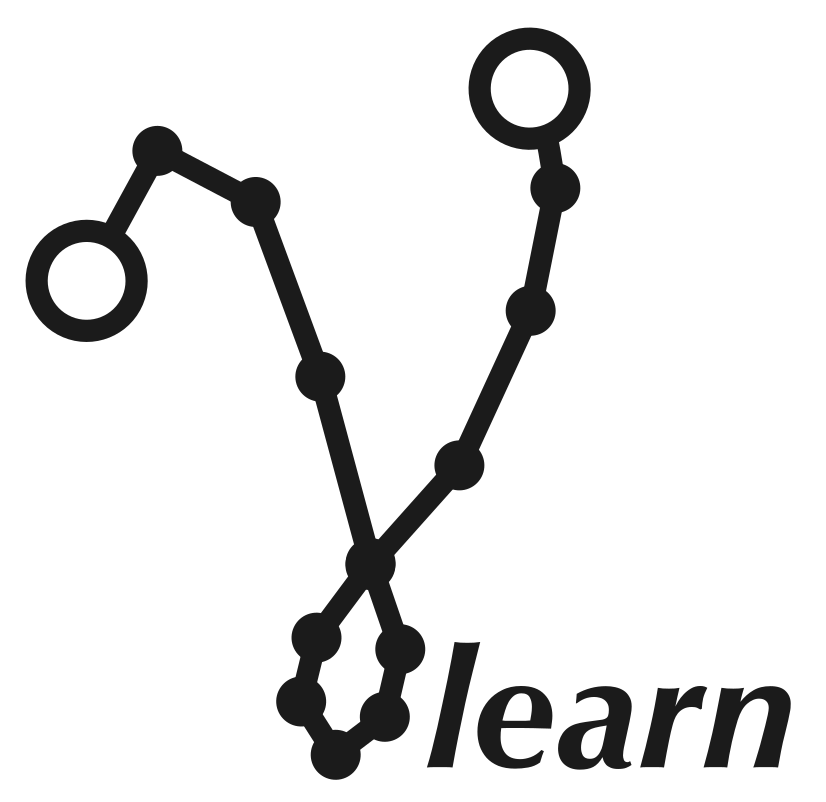
\includegraphics[height=0.55cm]{figures/logo_glearn_2020.png}\hspace*{.75cm}~%
        
\includegraphics[height=0.75cm]{figures/logo-Escape_0.png}
    \end{center}
}

\logo{
    
\includegraphics[width=0.1\linewidth]{figures/LogoIDEFICS_SANSbaseline_V.png}
}

%End of title page configuration block
%------------------------------------------------------------
%The next block of commands puts the table of contents at the 
%beginning of each section and highlights the current section:

% \AtBeginSection[]
% {
%   \begin{frame}
%     \frametitle{Table of Contents}
%     \tableofcontents[currentsection]
%   \end{frame}
% }
%------------------------------------------------------------
\begin{document}

\begingroup
\makeatletter
\setlength{\hoffset}{-.5\beamer@sidebarwidth}
\makeatother
\begin{frame}[plain]
    \titlepage
\end{frame}
\endgroup

%---------------------------------------------------------
% add some beamer settings that are different from the title page
\setbeamercolor{logo}{bg=white}
\addtobeamertemplate{navigation symbols}{}{%
    \usebeamerfont{footline}%
    \usebeamercolor[fg]{footline}%
    \hspace{1em}%
    \insertframenumber/\inserttotalframenumber
}

%-------------------------------------------------------------------------
%Highlighting text
% \begin{frame}
% \frametitle{Highlighting text}

% In this slide, some important text will be
% \alert{highlighted} because it's important.
% Please, don't abuse it.

% \begin{block}{Remark}
% Sample text
% \end{block}

% \begin{alertblock}{Important theorem}
% Sample text in red box
% \end{alertblock}

% \begin{examples}
% Sample text in green box. The title of the block is ``Examples".
% \end{examples}
% \end{frame}


%-------------------------------------------------------------------------

\section[Outline]{Objectives and outline}
    \begin{frame}{\secname}
        Goals of the lecture:
        \begin{itemize}
            \item Give a (narrow) overview of deep learning and its process
            \item Provide some keys to step in
            \item Explain into more details the fundamental components
            \item Experiment with widespread deep learning tools
        \end{itemize}
        At the end of the lecture, you should be able to:
        \begin{itemize}
            \item Design, implement and train a simple neural network
            \item Load a pretrained very deep network and fine tune it
        \end{itemize}
    \end{frame}
    
    \begin{frame}{\secname}
        Outline
        \begin{itemize}
            % \item Some elements of context
            \item Part I, Deep learning fundamentals
            \begin{itemize}
                \item Basic building blocks
                \item Training process
                \item Deep learning stack (hardware and software)
            \end{itemize}
            \item Part II, Going (really) deep
            \begin{itemize}
                \item Overview of famous very deep architectures
                \item Transfer learning: being lazy is good for the performance (and the planet)
                % \item Introduction to explainability
            \end{itemize}
            \item Wrap up and (some) further reflections
        \end{itemize}
    \end{frame}



%---------------------------------------------------------------------------
% \section[Context]{Context}
%     \subsection{A world of (big) data}
%     \begin{frame}{\secname}{\subsecname}
%         \begin{itemize}
%             \item Internet generates 2,500 Peta Bytes of data daily !
%         \end{itemize}
%         \begin{center}
%             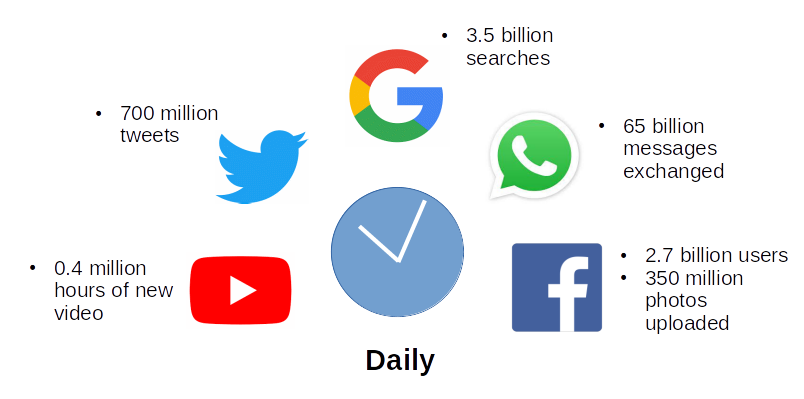
\includegraphics[width=0.9\linewidth]{figures/Context/big_data.png}
%         \end{center}
        
%         {\footnotesize
%         \cite{saasscout}, \cite{petrov2021techjury}, \cite{omnicore} 
%         }
%     \end{frame}
%     \begin{frame}{\secname}{\subsecname}
%         But also (scientific) specific fields:
%         \begin{itemize}
%             \item Medical imaging (43 million MRI scans in Europe in 2017 \cite{euhealthcare})
%             \item Remote sensing (Sentinel satellites provide hundreds of GB of data / year)
%             \item Astronomy
%             \begin{itemize}
%                 \item Gamma astronomy (CTA will generate 210 PB of data / year \cite{cta})
%                 \item Vera C. Rubin Observatory will produce 10 TB of data / night for 10 years \cite{lsst}
%             \end{itemize}
%             \item and many other domains \dots
%         \end{itemize}
%         % \begin{alertblock}{}
%         %     We need machine learning to process these big data
%         % \end{alertblock}
%     \end{frame}
%     \begin{frame}{\secname}{\subsecname}
%         From these data, we want:
%         \begin{itemize}
%             \item To sell advertises (18 billion \$ revenue for Facebook between April and June 2020 \cite{facebook})
%             \item Our cars to self-drive
%             \item To help doctors identify disease
%             \item To improve agriculture
%             \item To better understand the Universe
%             \item \dots
%         \end{itemize}
%         \begin{alertblock}{}
%             We need machine learning to process these big data
%         \end{alertblock}
%     \end{frame}
    
%     \subsection[Machine learning]{Machine learning, a quick reminder}
%     \begin{frame}{\secname}{\subsecname}
%         % ML concepts to end up with the specificity of DL
%         Machine learning = algorithms learn to solve tasks
%         \begin{center}
%             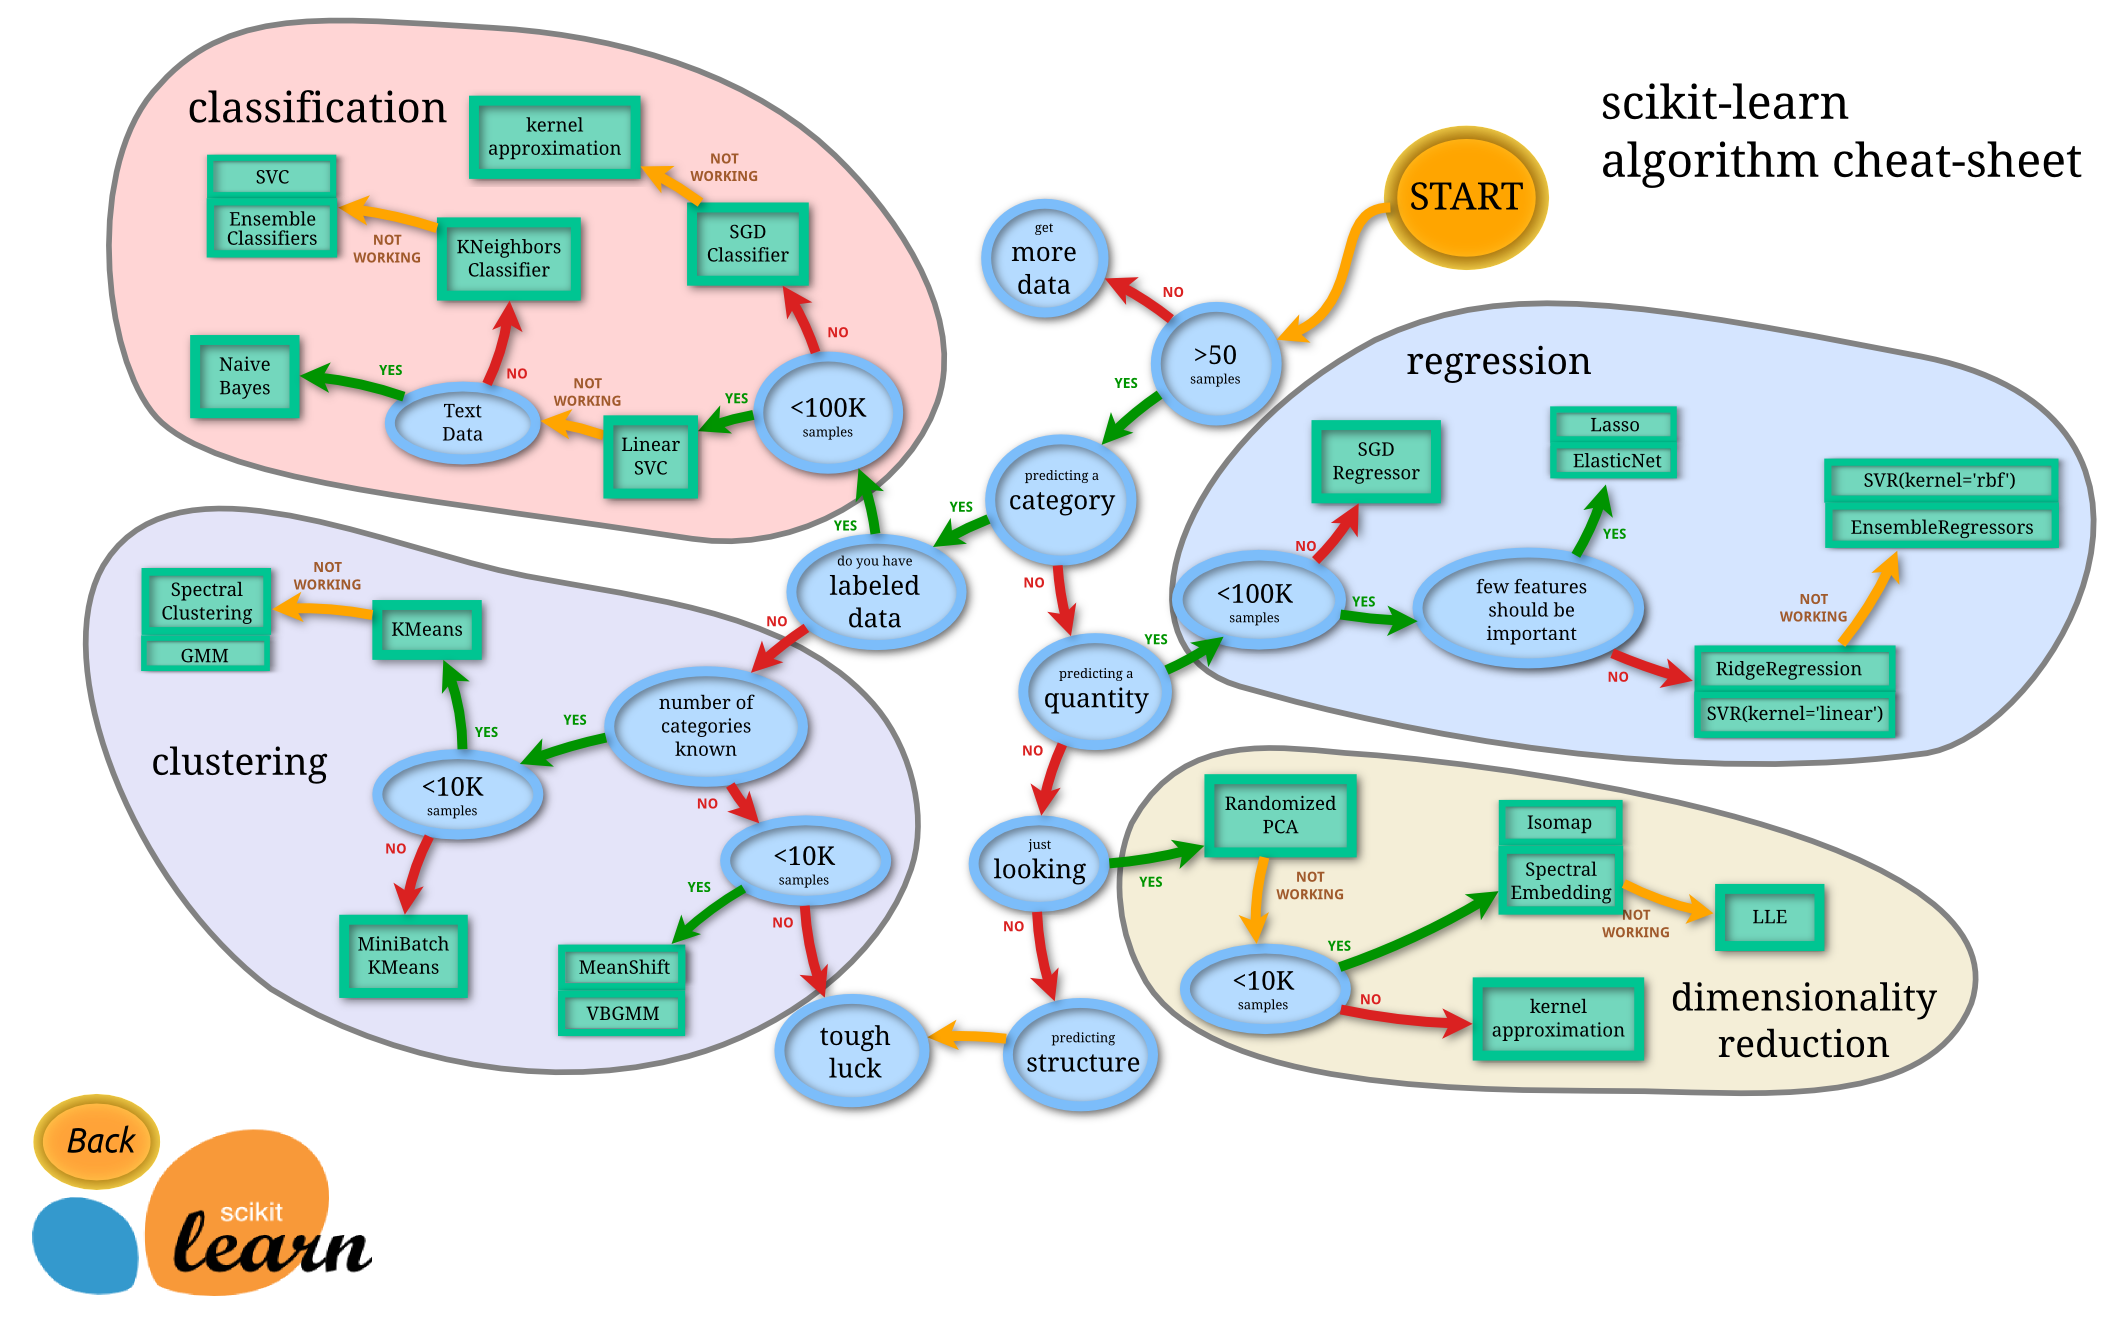
\includegraphics[width=0.9\linewidth]{figures/Context/scikit-learn_ml_map.png}
%             Supervised vs Unsupervised
%         \end{center}
%     \end{frame}
%     \begin{frame}{\secname}{\subsecname}
%         % ML concepts to end up with the specificity of DL
%         Machine learning principle
%         \begin{center}
%             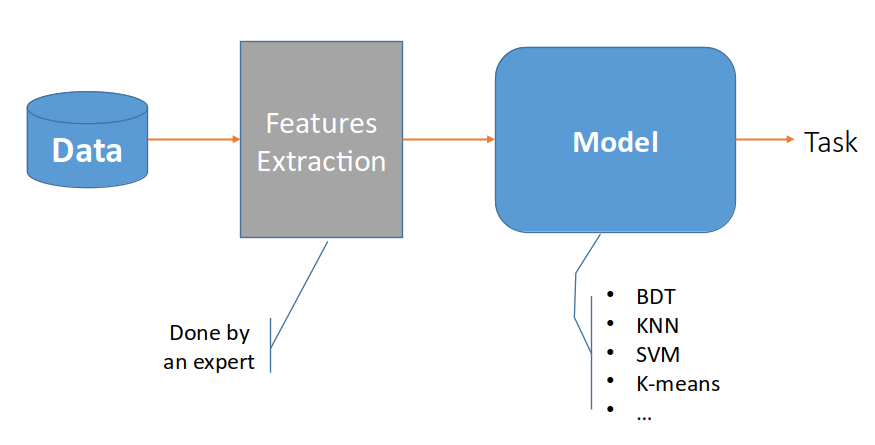
\includegraphics[width=\linewidth]{figures/Context/ML_principle.png}
%         \end{center}
%     \end{frame}
%     \begin{frame}{\secname}{\subsecname}
%         % ML concepts to end up with the specificity of DL
%         \sout{Machine} learning principle
        
%         \alert{Deep}
%         \begin{center}
%             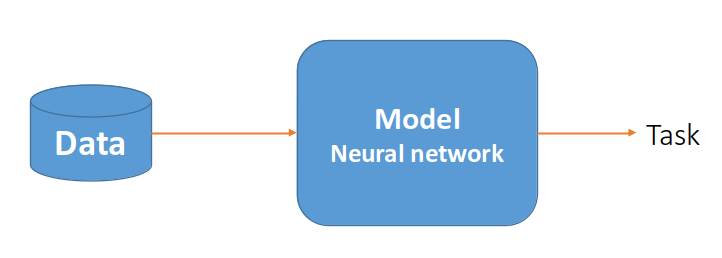
\includegraphics[width=0.82\linewidth]{figures/Context/DL_principle.png}
%         \end{center}
%         \begin{itemize}
%             \item The features are learned by the model
%             \item Search for regularity with an over-parametrized model within large sets of data
%         \end{itemize}
%     \end{frame}
    
    

% %----------------------------------------------------------------------------
\section[DL Fundamentals]{Part I, Deep Learning fundamentals}
    
    \begin{frame}{\secname}
        \begin{block}{Disclaimer}
            In this lecture, we mainly focus on:
            \begin{itemize}
                \item Computer vision tasks and models
                \item Supervised learning (classification and regression)
            \end{itemize}
            But the techniques presented are fully applicable to other fields / learning methods.\\
            In the following, important \alert{vocabulary} will be highlighted in red.
        \end{block}
    \end{frame}
    \begin{frame}{\secname}
        Outline
        \begin{itemize}
            \item A bit of history
            \item Building deep neural networks
            \item Training deep neural networks
            \item Deep learning libraries
            \item First hands on session
        \end{itemize}
    \end{frame}
    \begin{frame}{\secname}
        Spoiler alert ! This is \textbf{not} the current state of AI / DL
        \begin{center}
            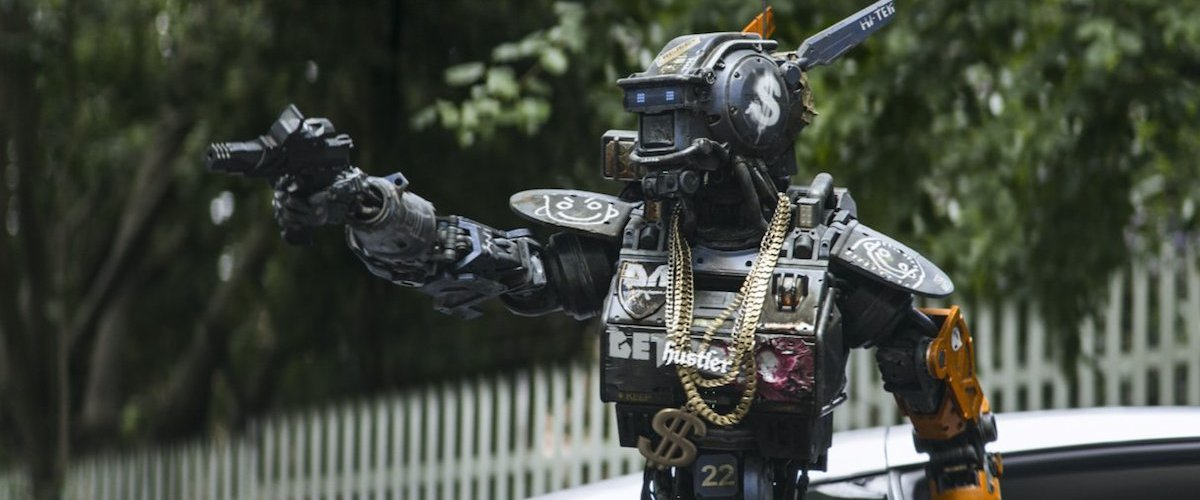
\includegraphics[width=0.8\linewidth]{figures/DL_fundamentals/Chappie_2015_1.jpg}
            {\tiny Chappie, 2015}
        \end{center}
        \begin{itemize}
            \item DL is far from human-level AI
            \item It lacks:
            \begin{itemize}
                \item Generalization
                \item Causality
                \item Logical reasonning
            \end{itemize}
        \end{itemize}
    \end{frame}
    \begin{frame}{\secname}
        \begin{itemize}
            \item DL outperforms humans on \textbf{specific and narrow} tasks
        \end{itemize}
        \begin{center}
            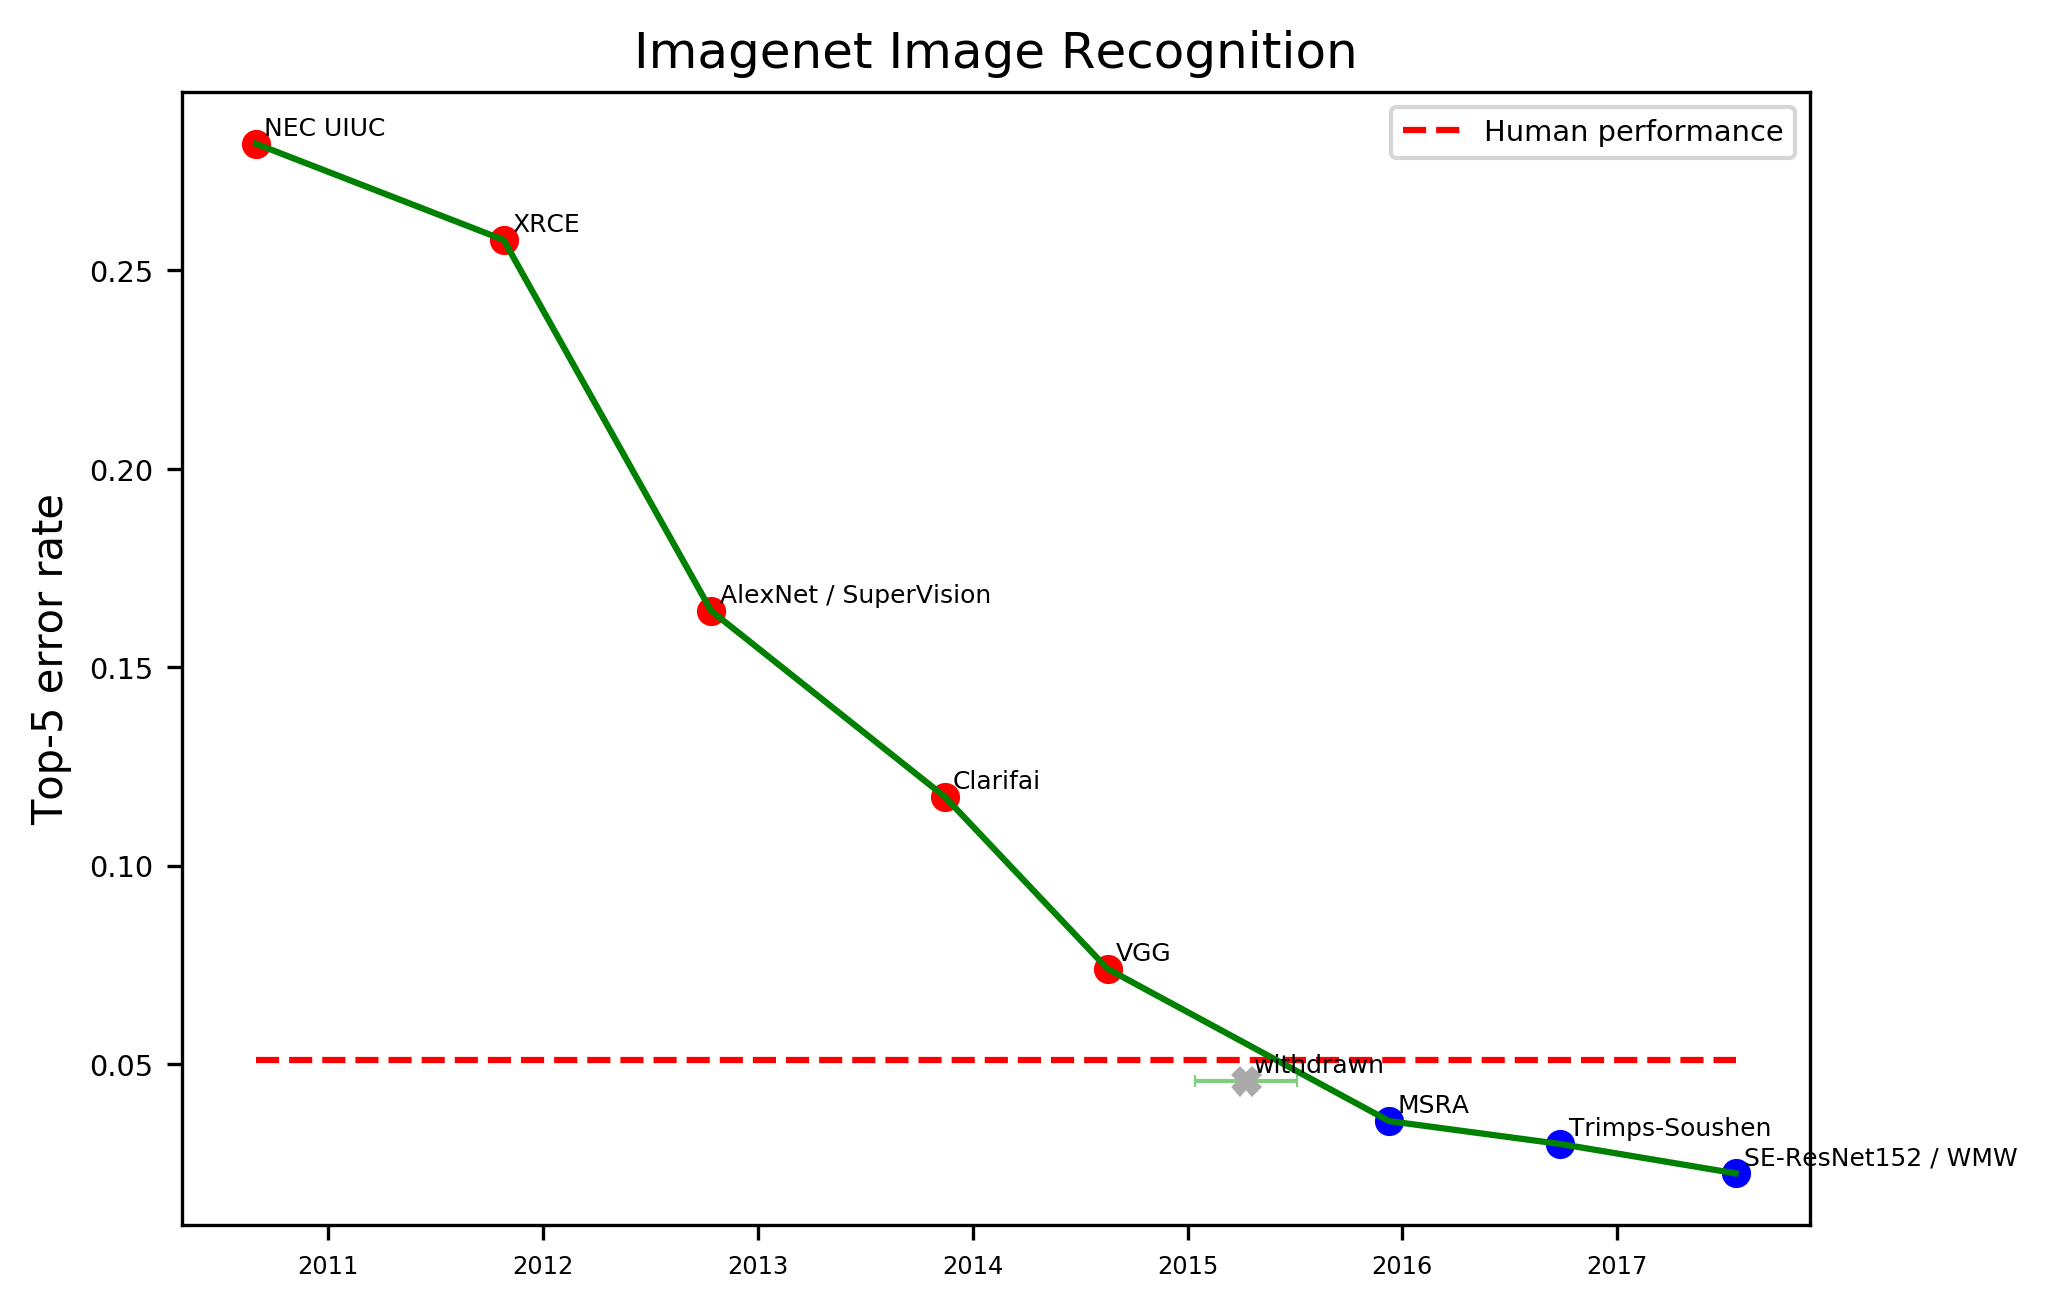
\includegraphics[width=\linewidth]{figures/DL_fundamentals/imagenet_perf.png}
        \end{center}
    \end{frame}
    \begin{frame}{\secname}
        \begin{itemize}
            \item DL outperforms humans on \textbf{specific and narrow} tasks
        \end{itemize}
        \begin{center}
            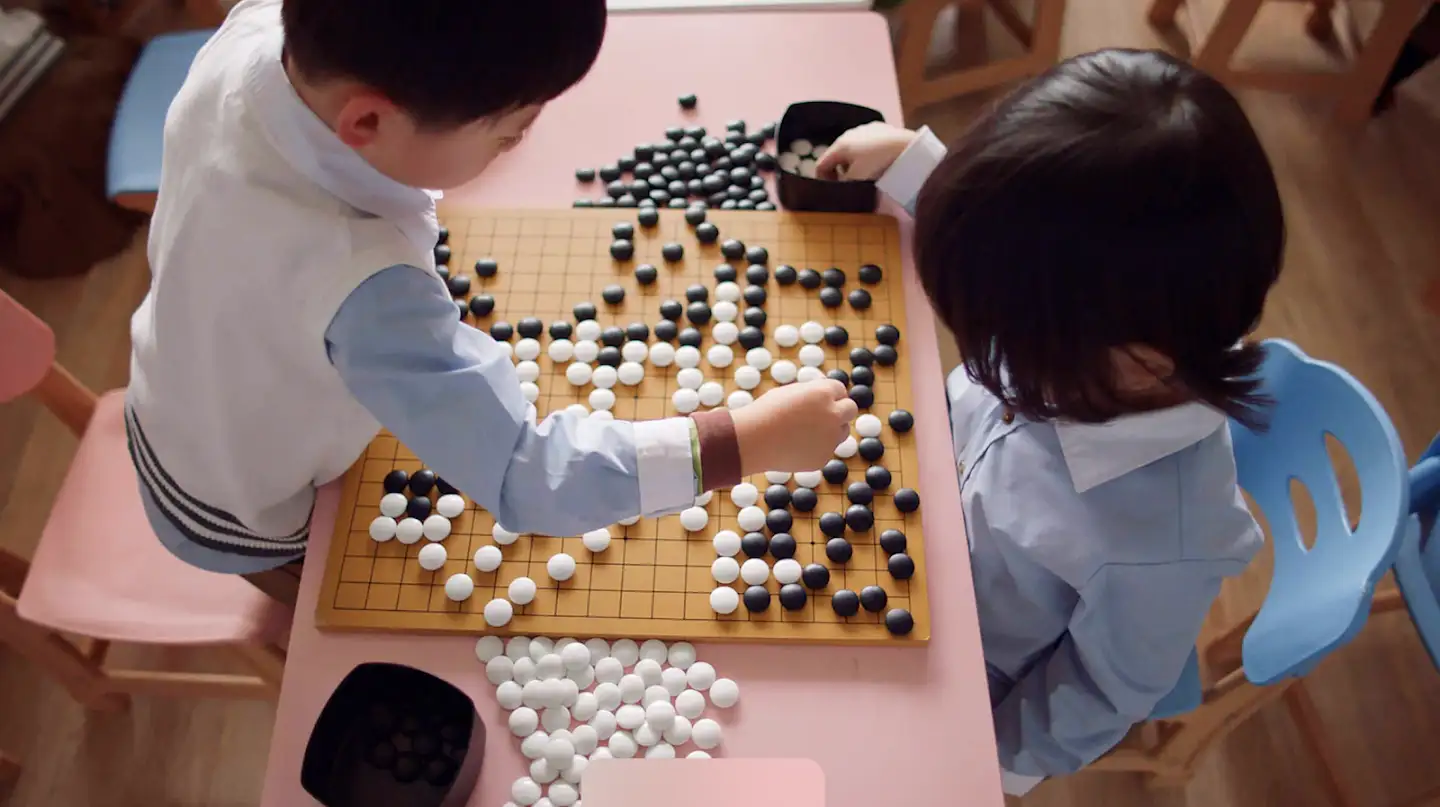
\includegraphics[width=0.75\linewidth]{figures/DL_fundamentals/alphago_ex.png}
            
\includegraphics[width=0.2\linewidth]{figures/DL_fundamentals/Alphago_logo.png}
        \end{center}
    \end{frame}
    \begin{frame}{\secname}
        \begin{itemize}
            \item DL outperforms humans on \textbf{specific and narrow} tasks
        \end{itemize}
        \begin{center}
            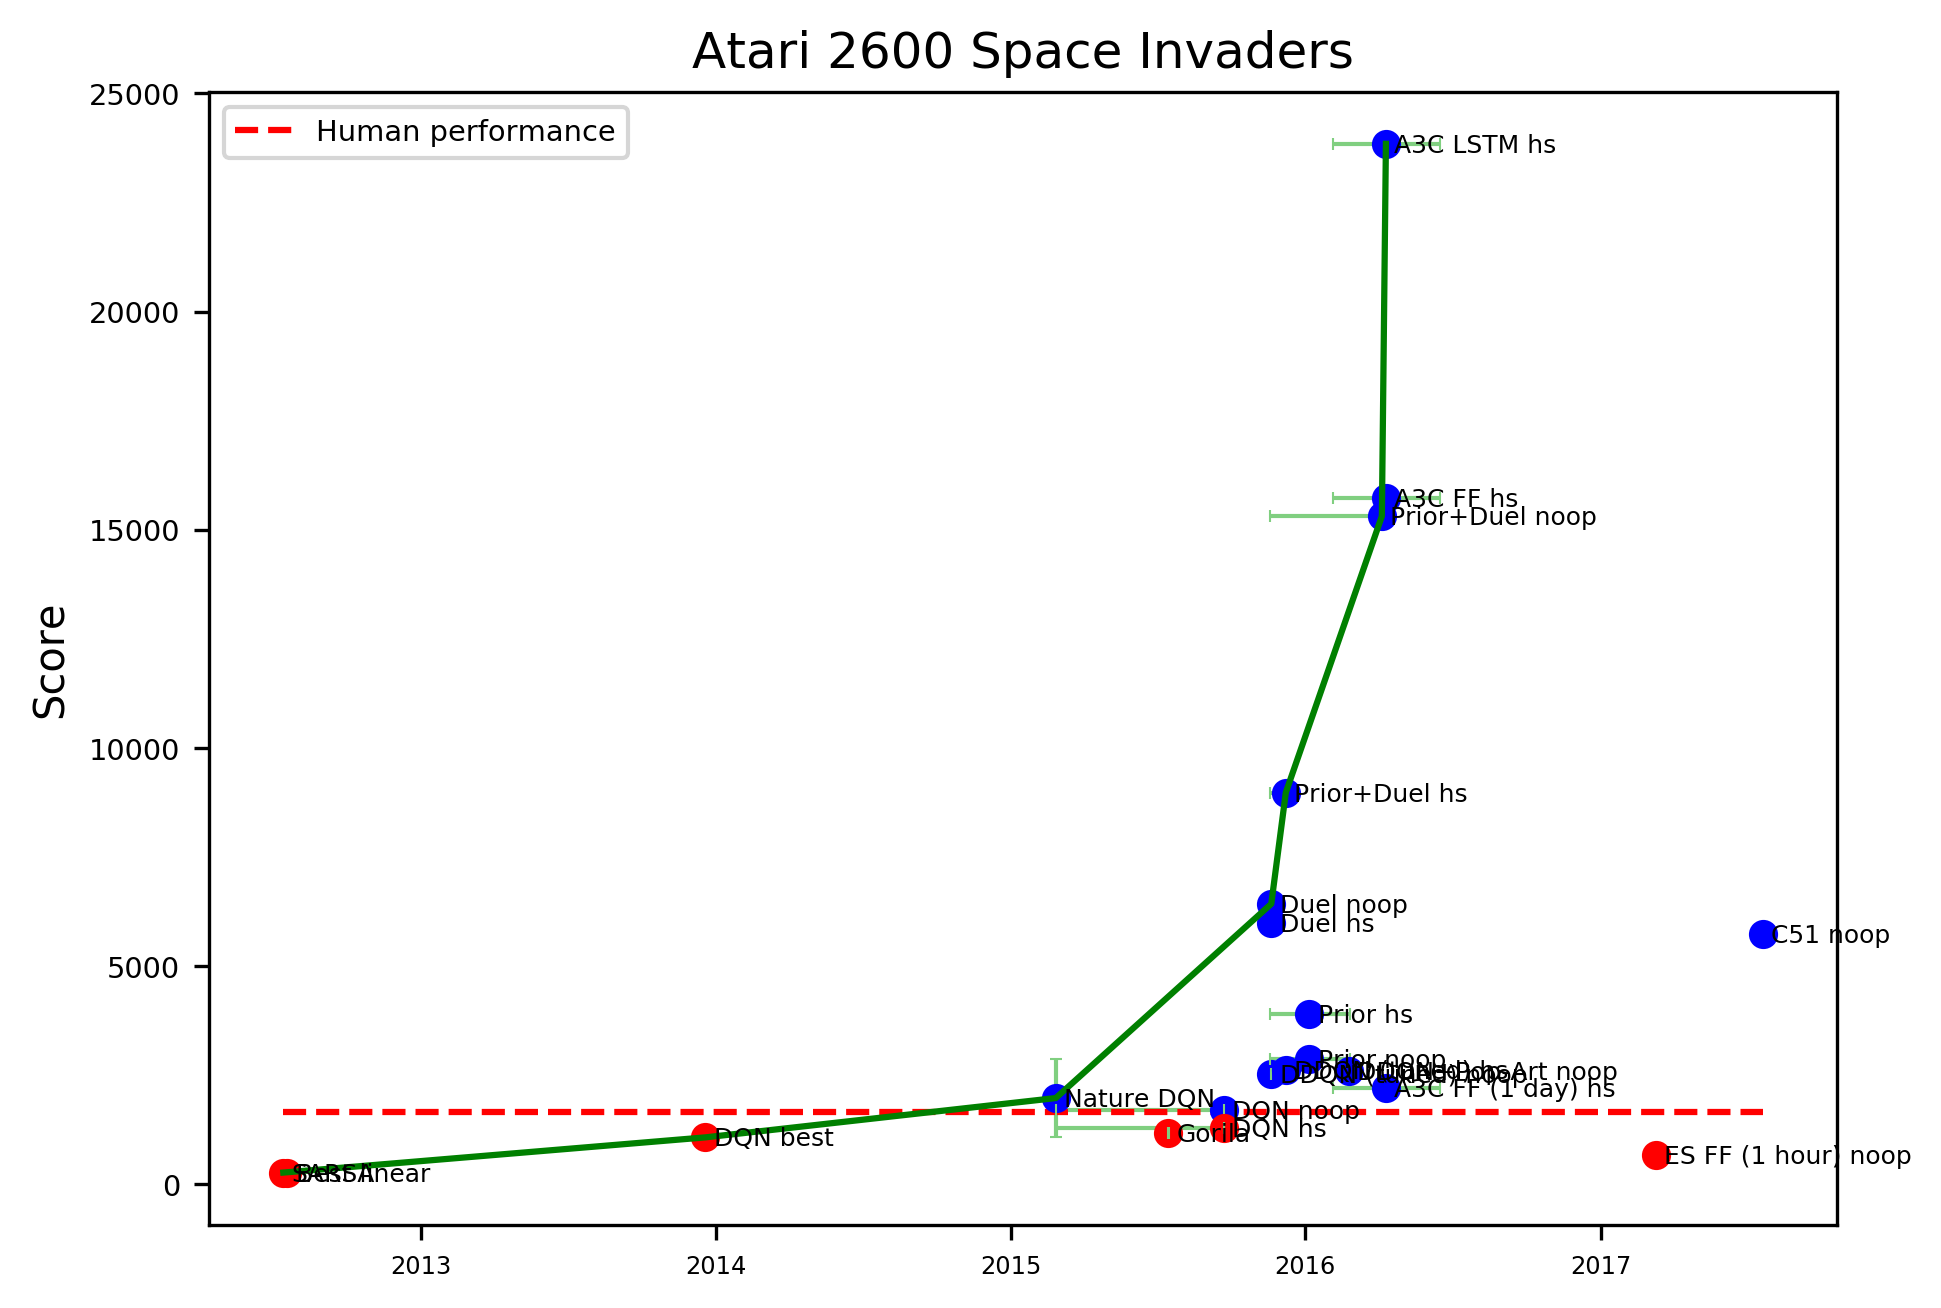
\includegraphics[width=\linewidth]{figures/DL_fundamentals/space_invader_perf.png}
        \end{center}
    \end{frame}
    \begin{frame}{\secname}
        \begin{itemize}
            \item DL outperforms humans on \textbf{specific and narrow} tasks
        \end{itemize}
        \begin{center}
            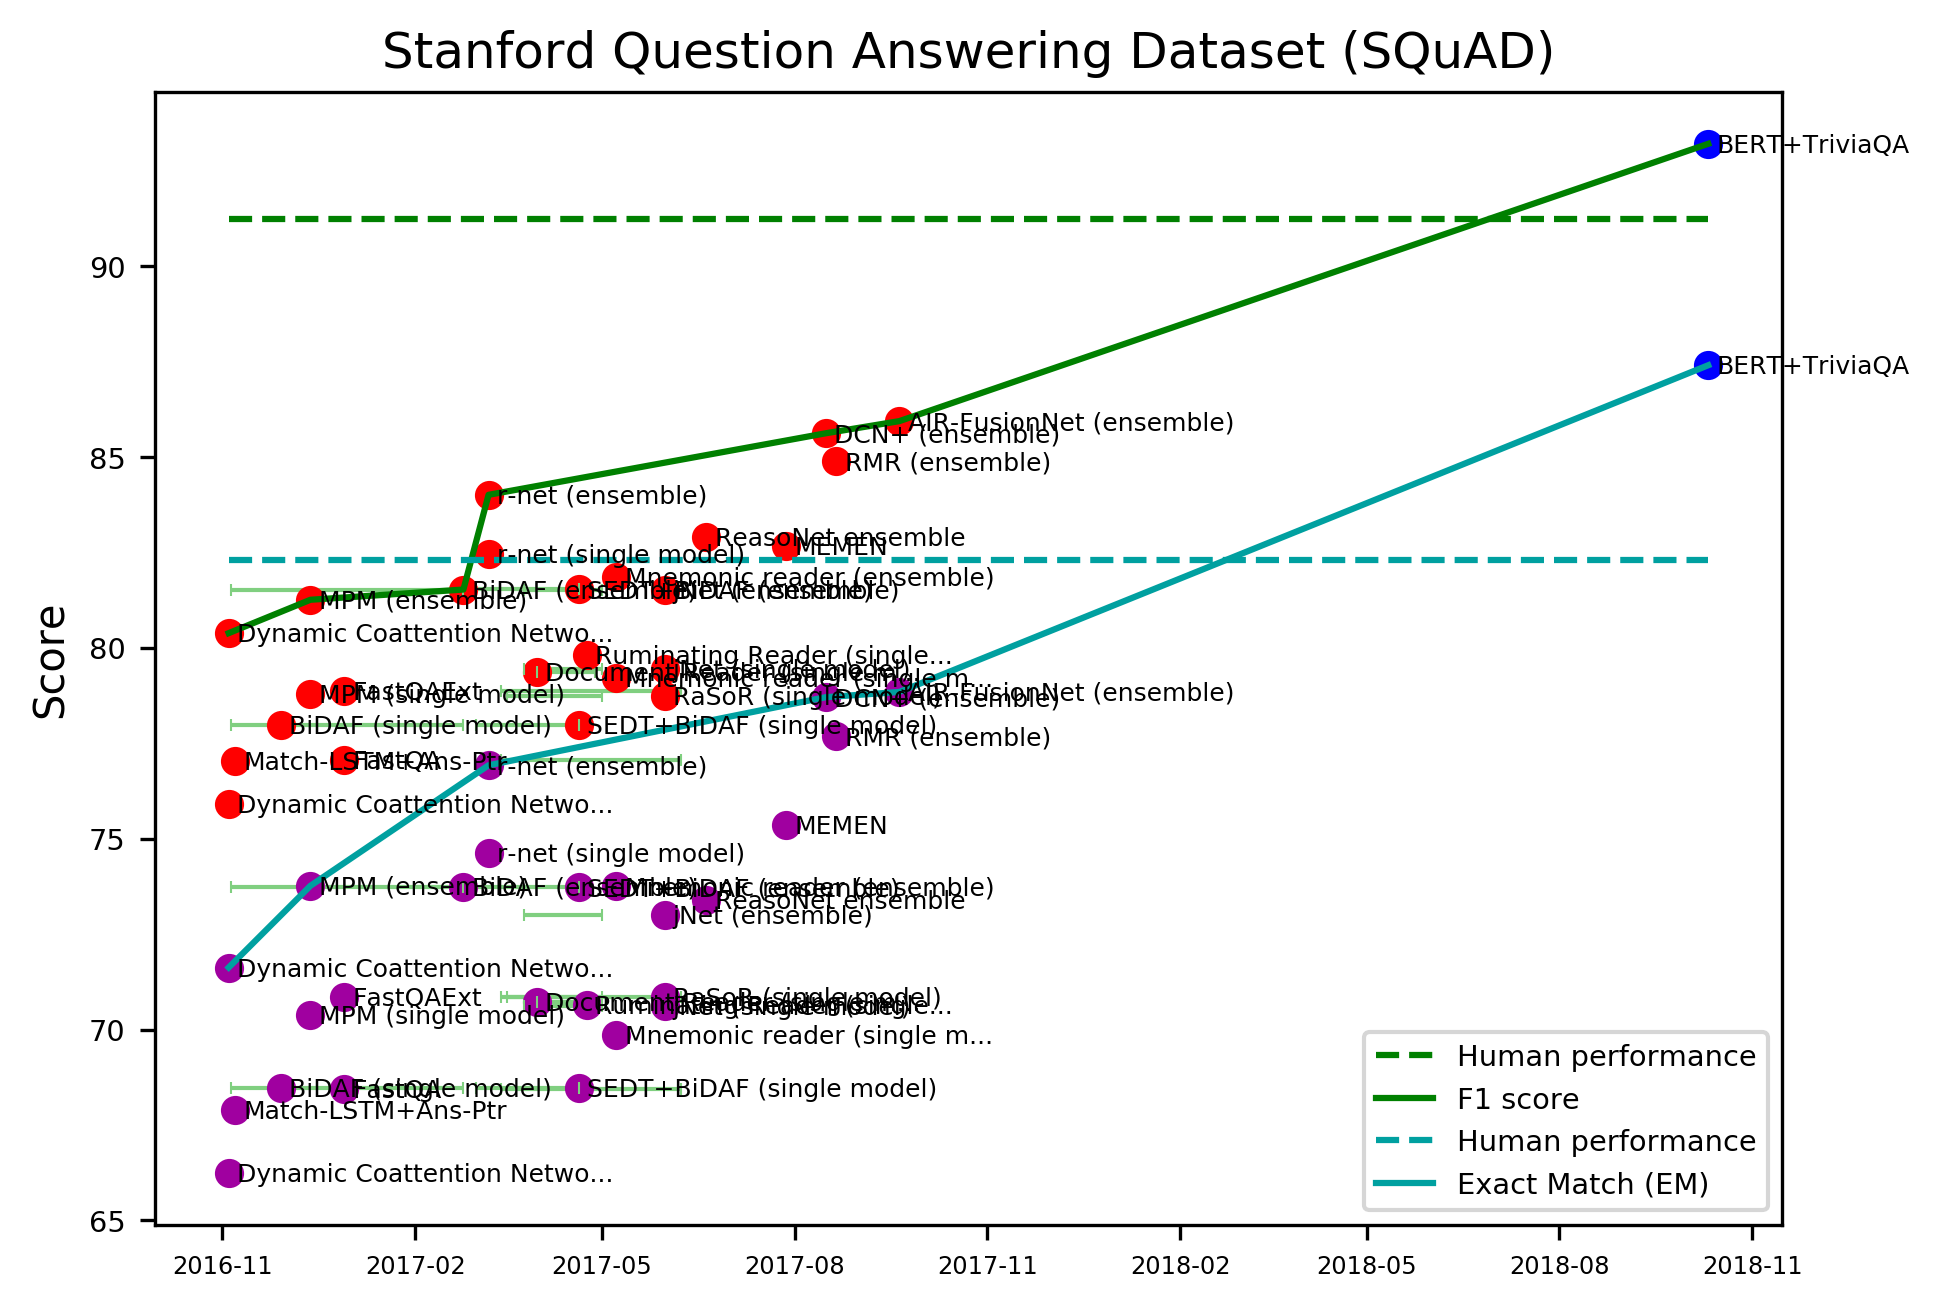
\includegraphics[width=\linewidth]{figures/DL_fundamentals/stanford_QA_perf.png}
        \end{center}
    \end{frame}
    \begin{frame}{\secname}
        \begin{itemize}
            \item DL outperforms humans on \textbf{specific and narrow} tasks
        \end{itemize}
        \begin{center}
            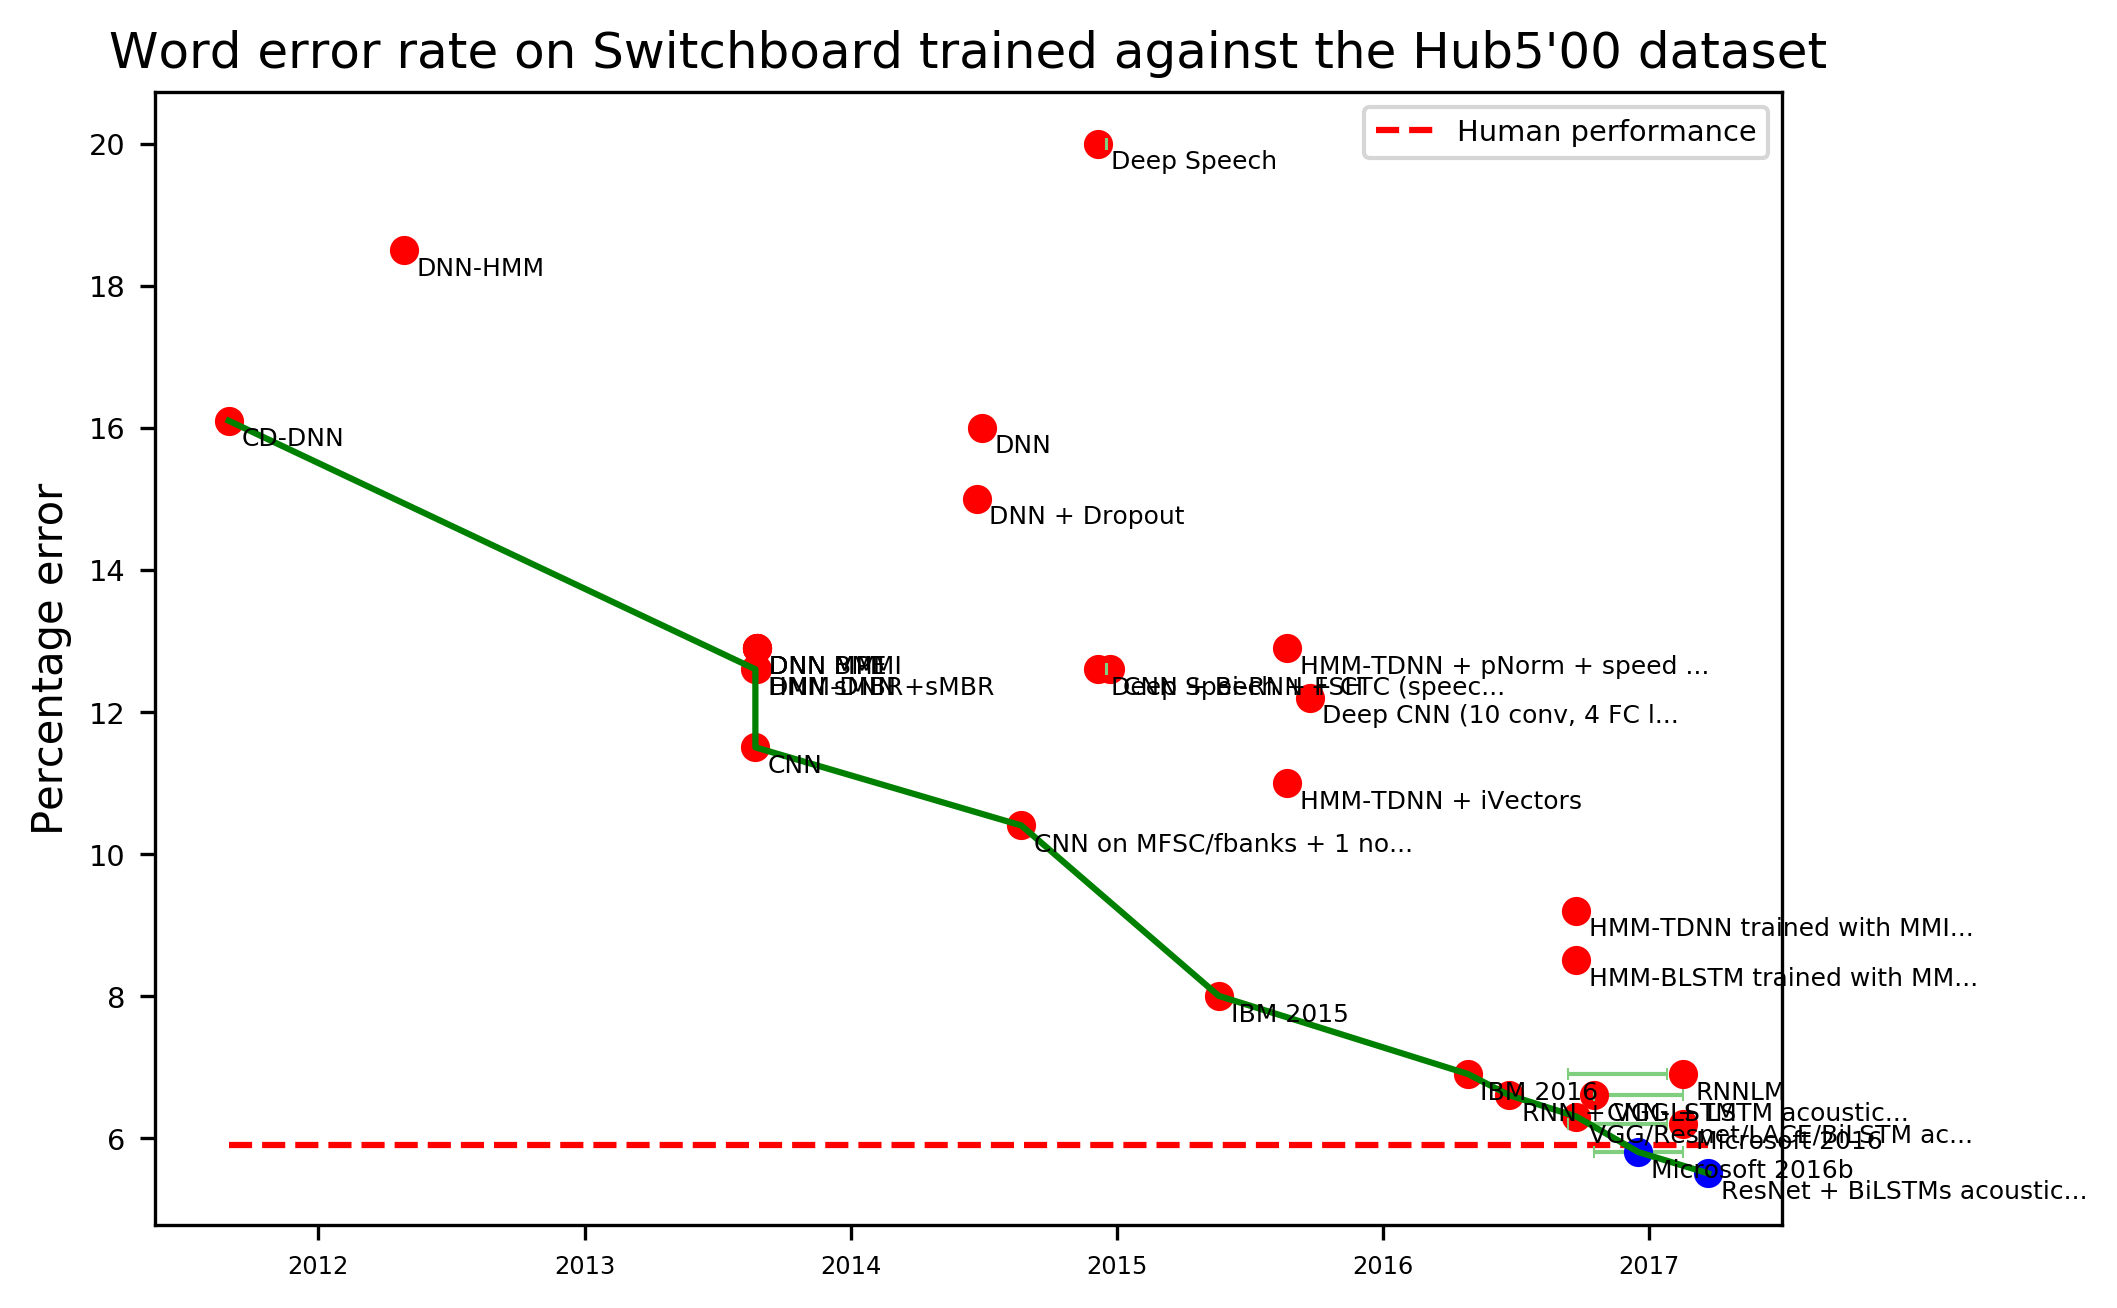
\includegraphics[width=0.9\linewidth]{figures/DL_fundamentals/speech_recog_perf.png}
            \vspace{-0.7em}
            {\tiny \href{https://www.eff.org/ai/metrics}{Source}}
        \end{center}
    \end{frame}
    % \begin{frame}{\secname}
    %     \begin{itemize}
    %         \item DL outperforms humans on \textbf{specific and narrow} tasks
    %     \end{itemize}
    %     \begin{center}
    %         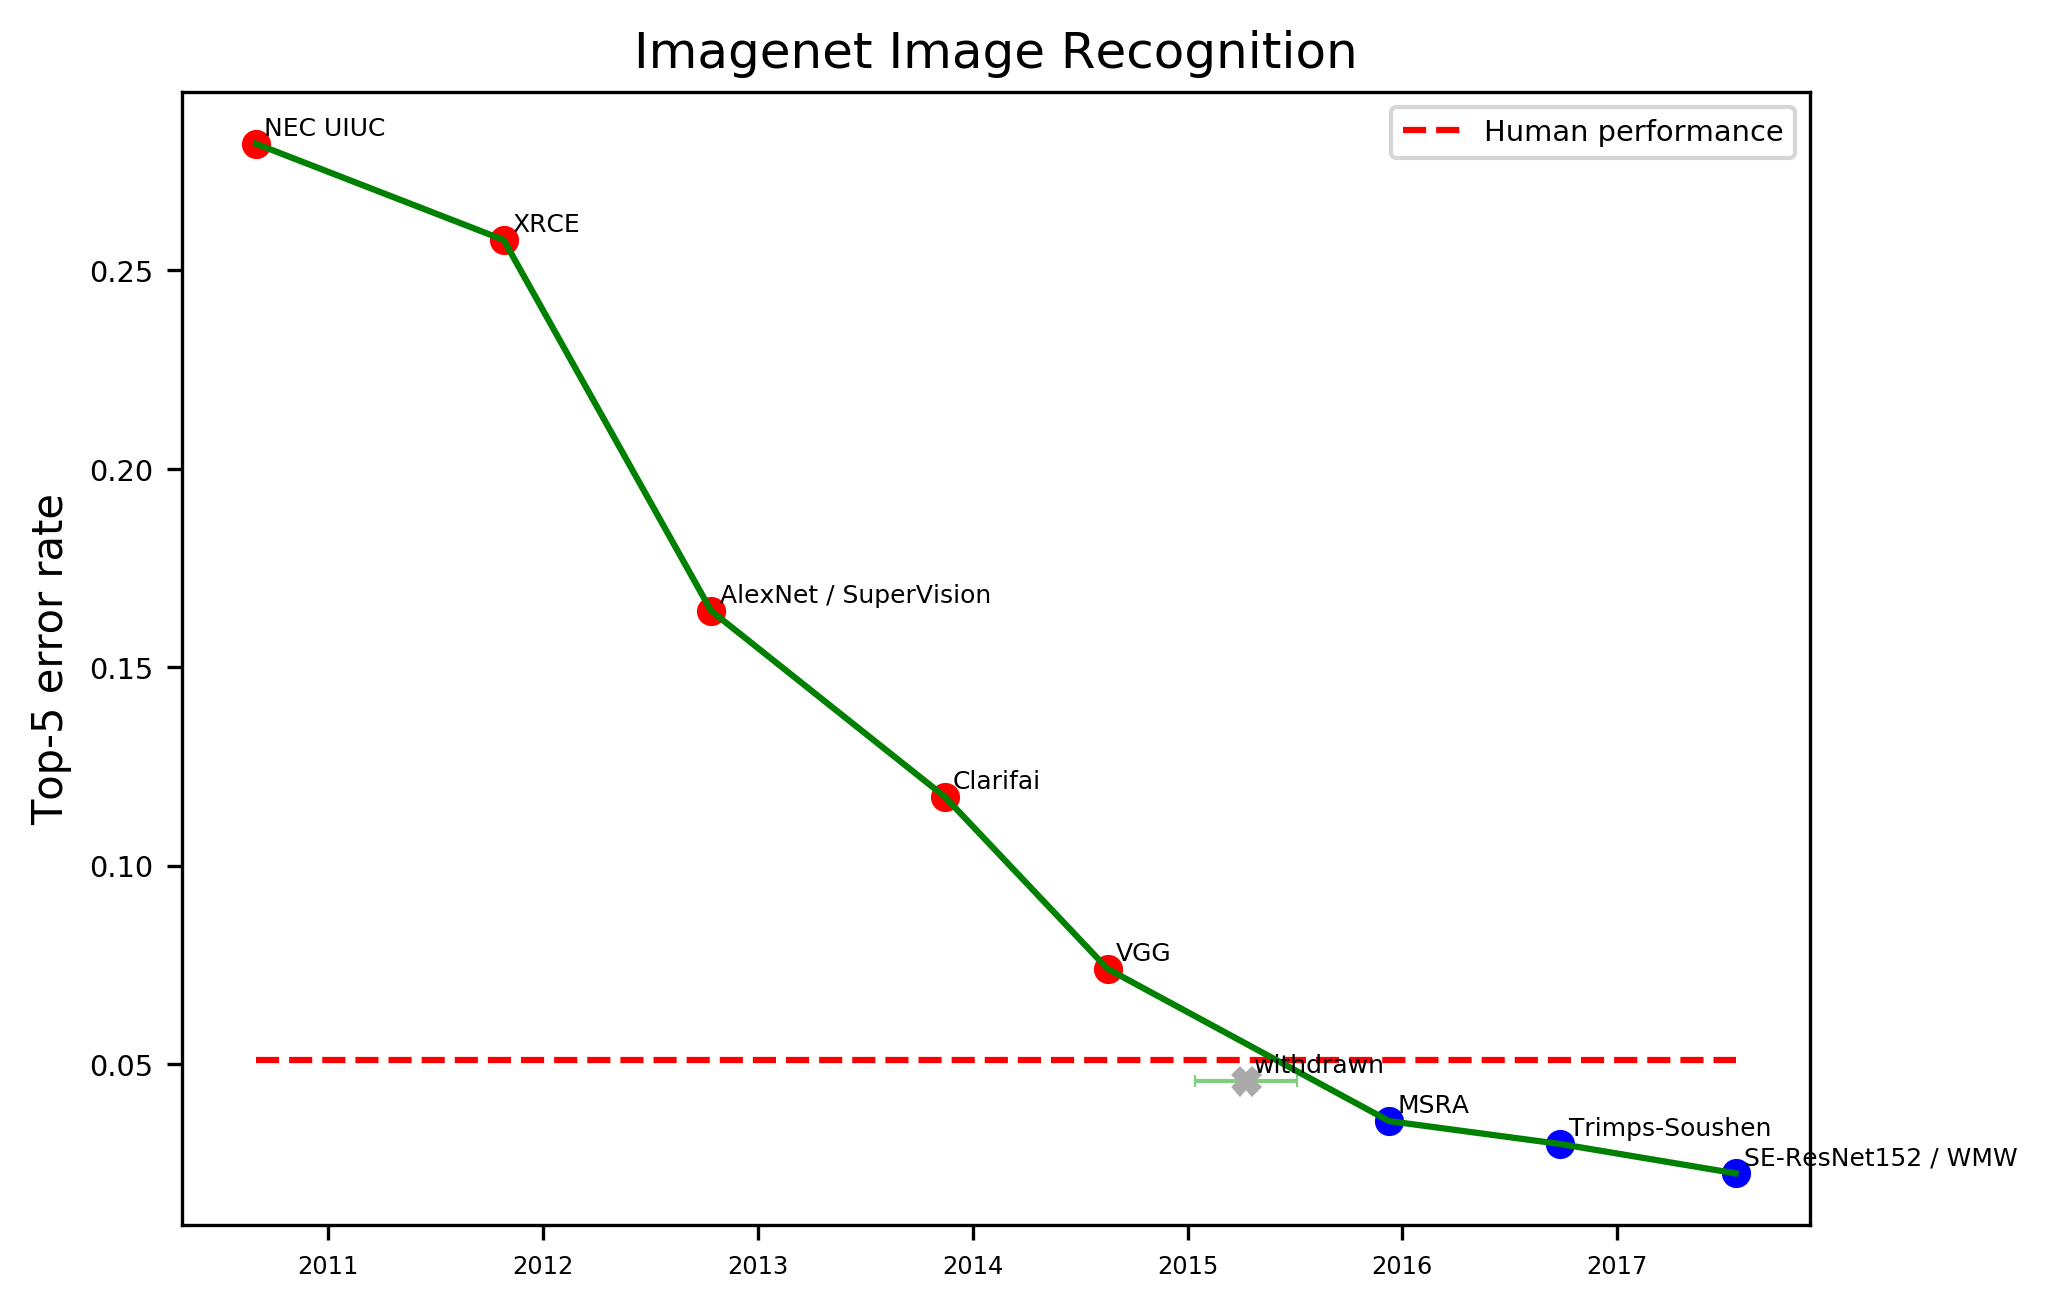
\includegraphics[width=0.5\linewidth]{figures/DL_fundamentals/imagenet_perf.png}
    %         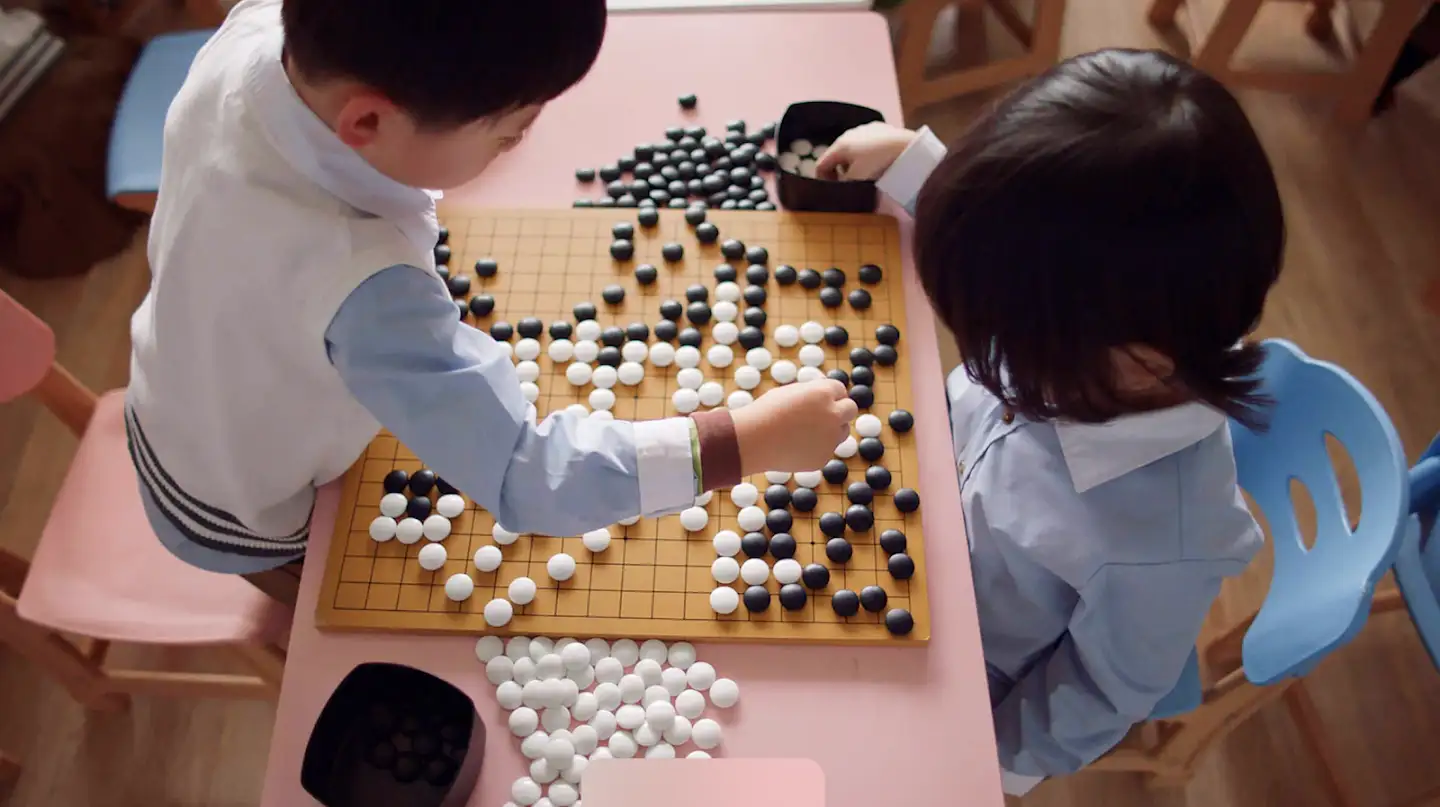
\includegraphics[width=0.5\linewidth]{figures/DL_fundamentals/alphago_ex.png}
    %         
\includegraphics[width=0.2\linewidth]{figures/DL_fundamentals/Alphago_logo.png}
    %         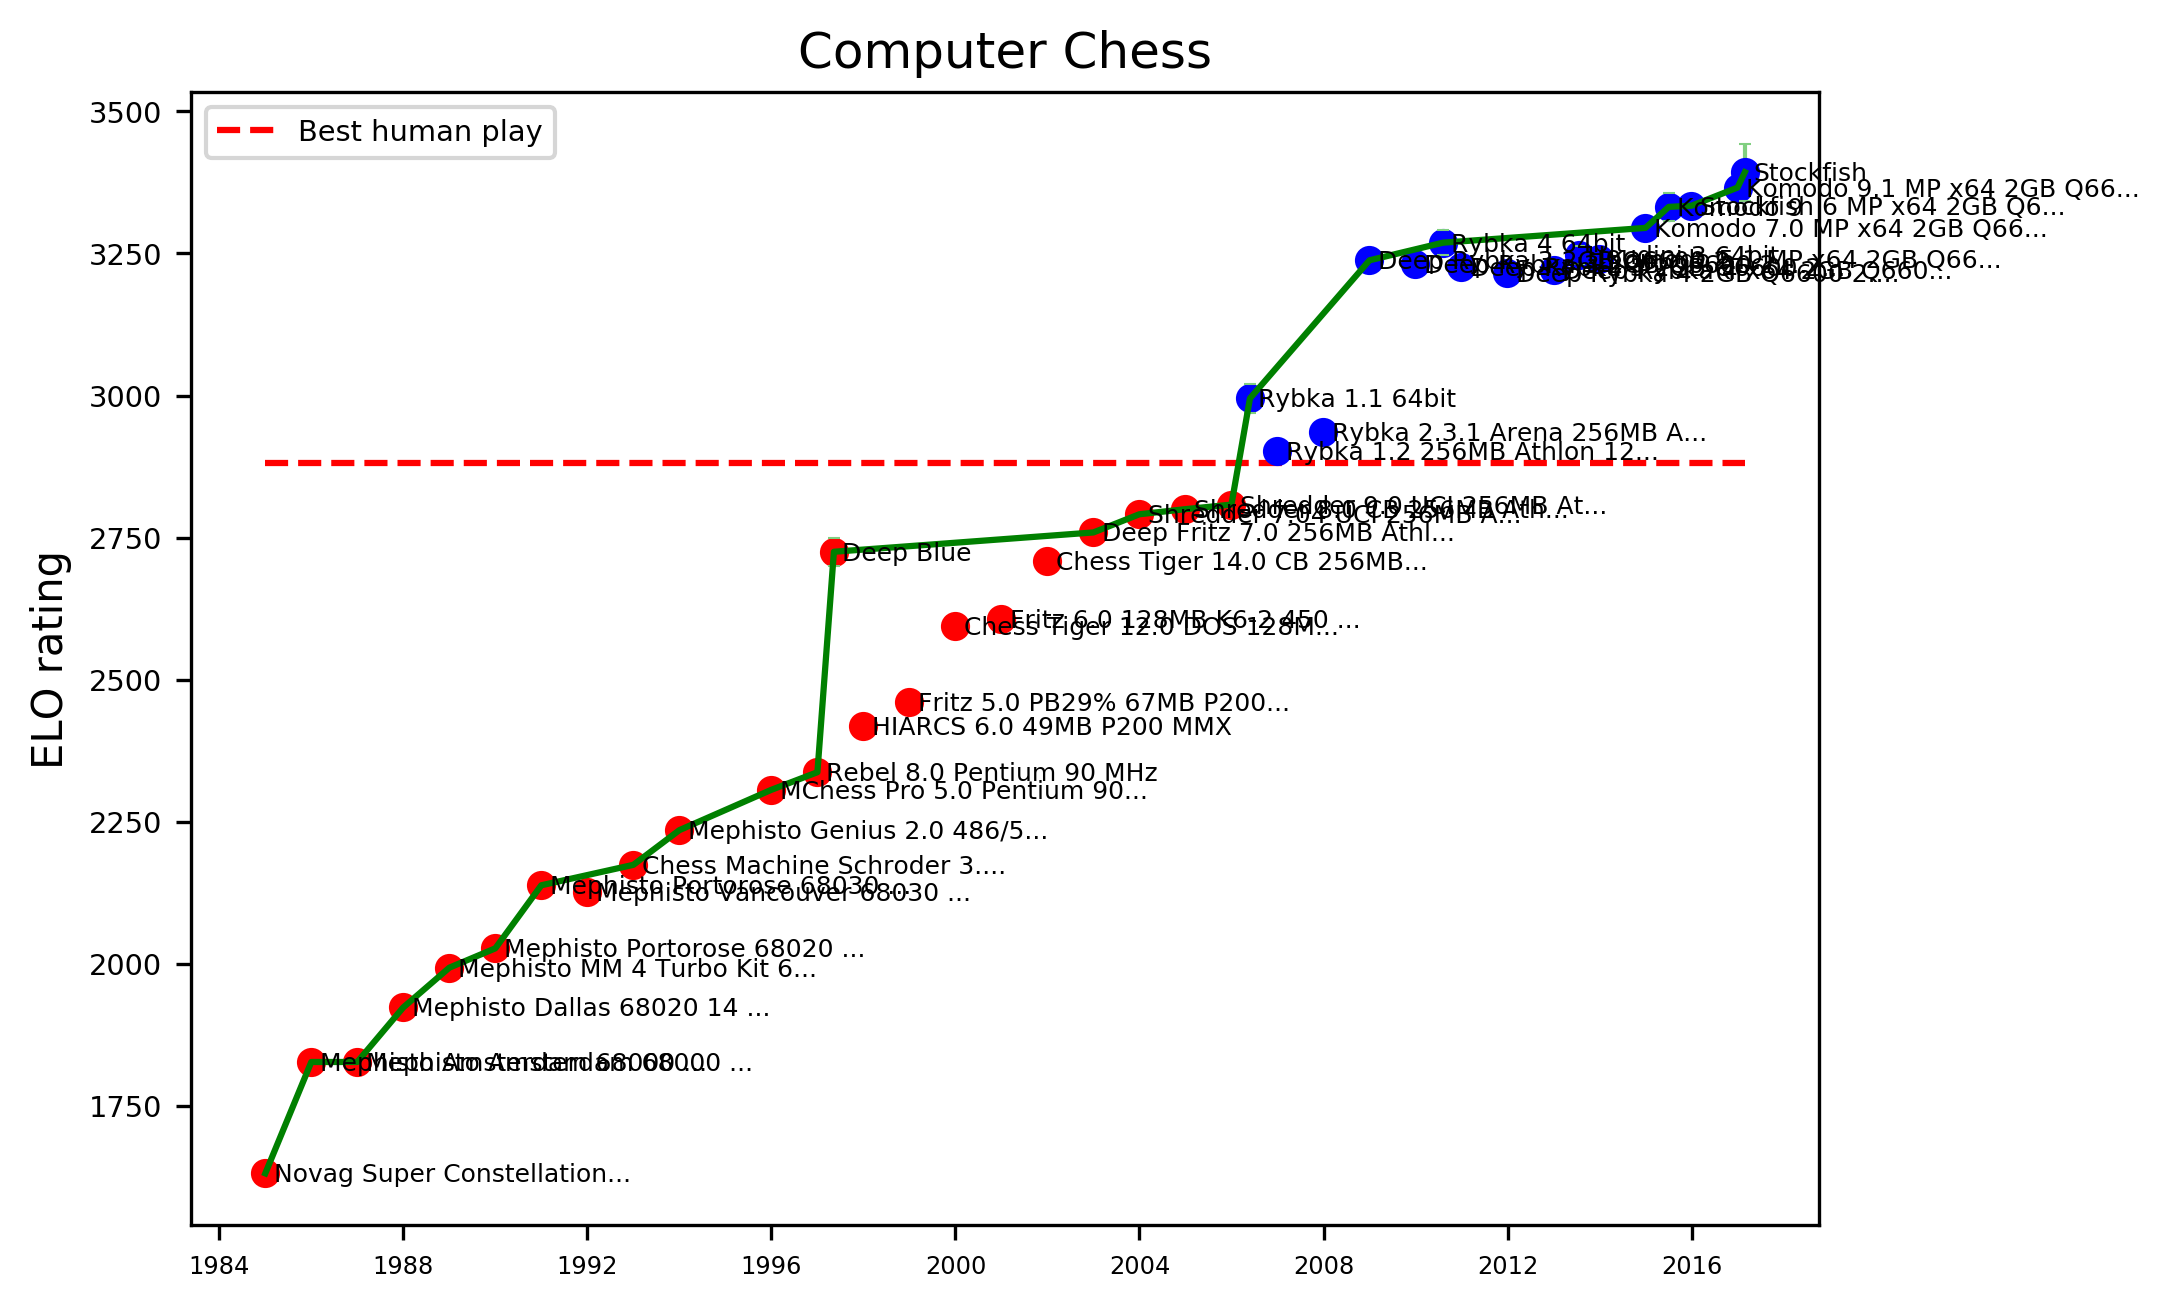
\includegraphics[width=0.5\linewidth]{figures/DL_fundamentals/chess_perf.png}
    %         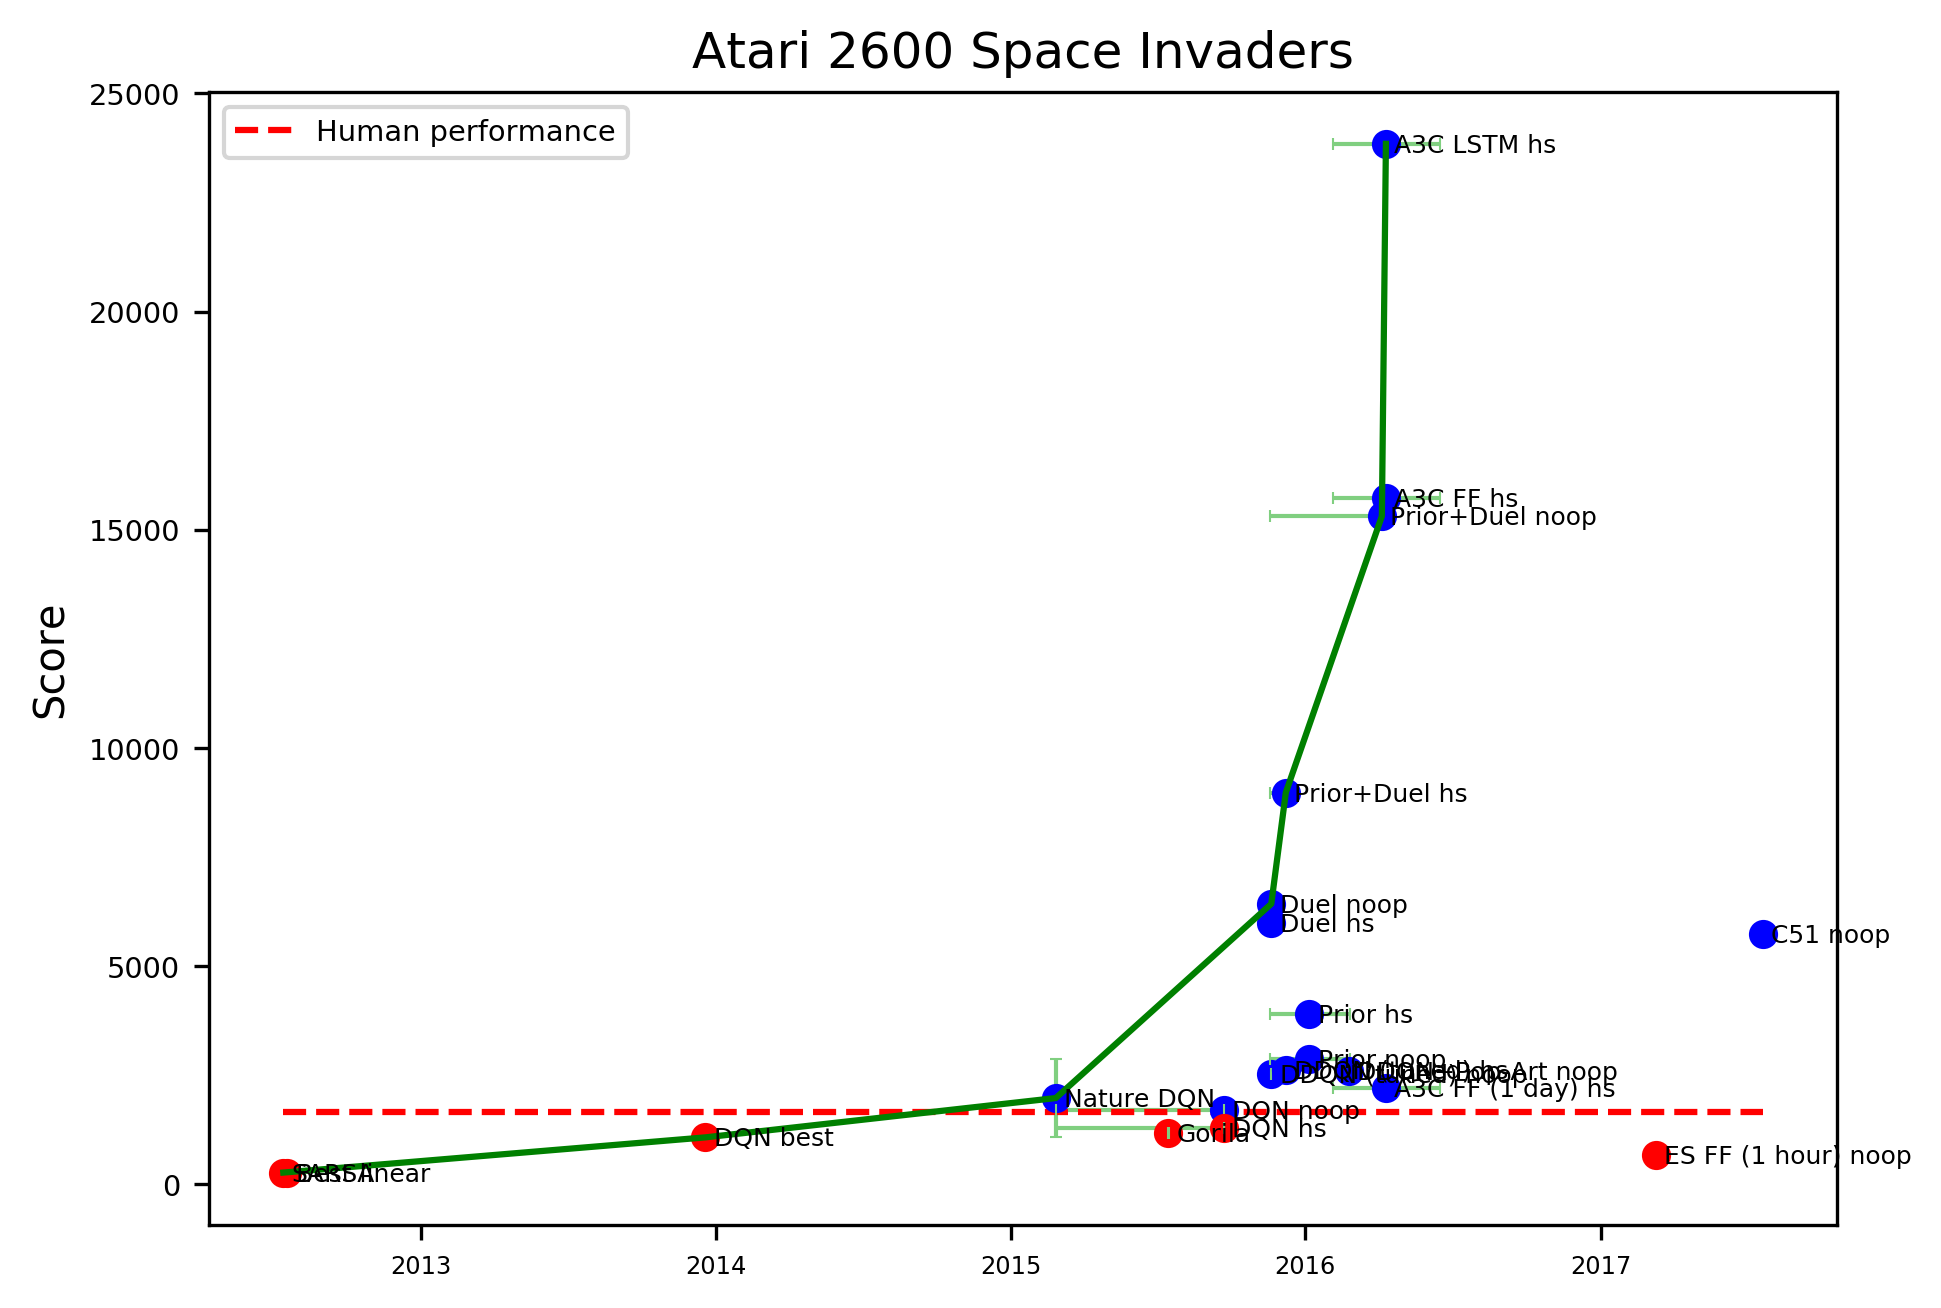
\includegraphics[width=0.5\linewidth]{figures/DL_fundamentals/space_invader_perf.png}
    %         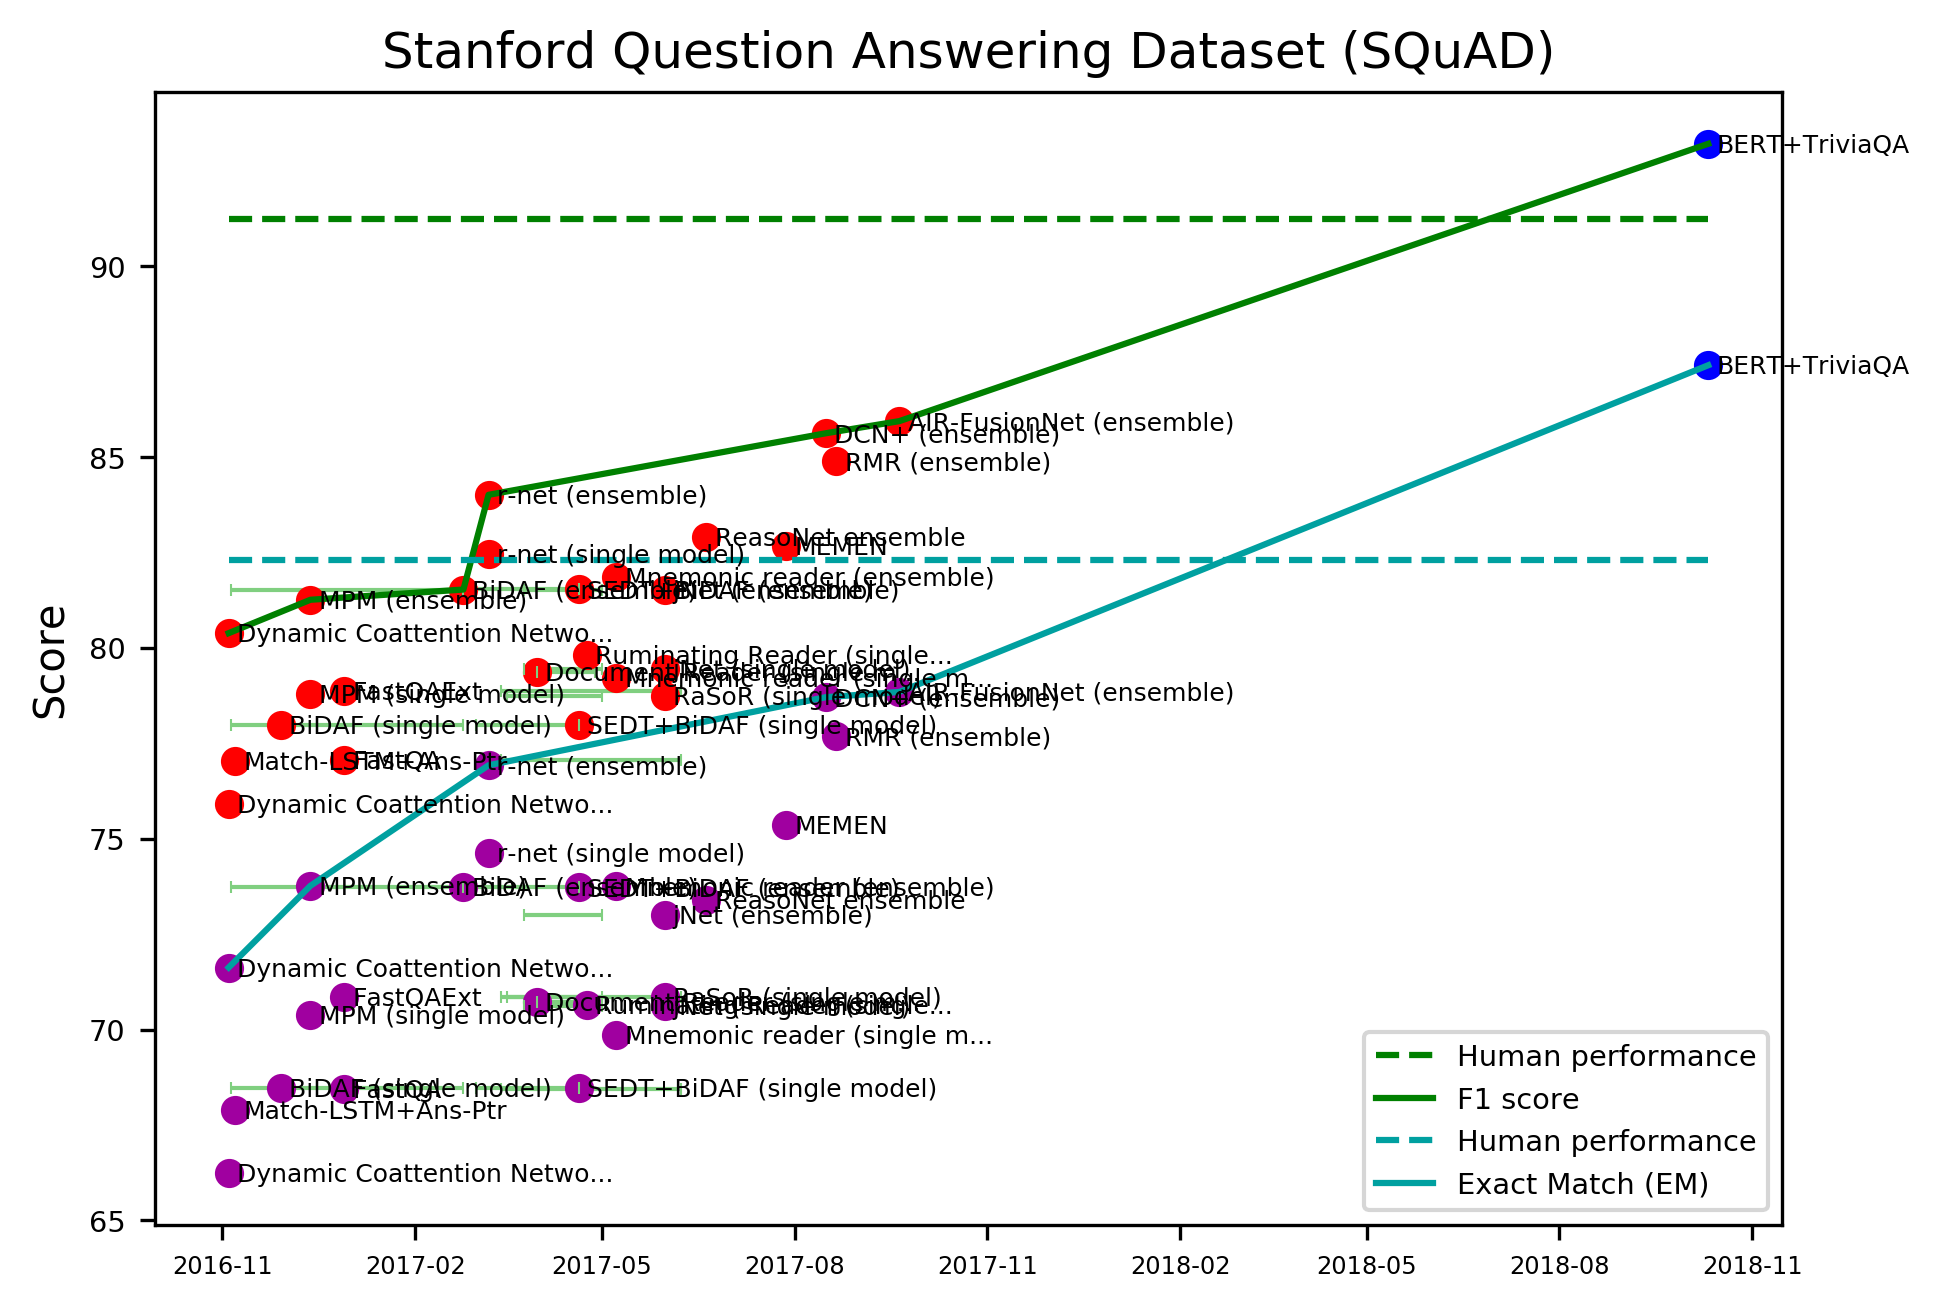
\includegraphics[width=0.5\linewidth]{figures/DL_fundamentals/stanford_QA_perf.png}
    %         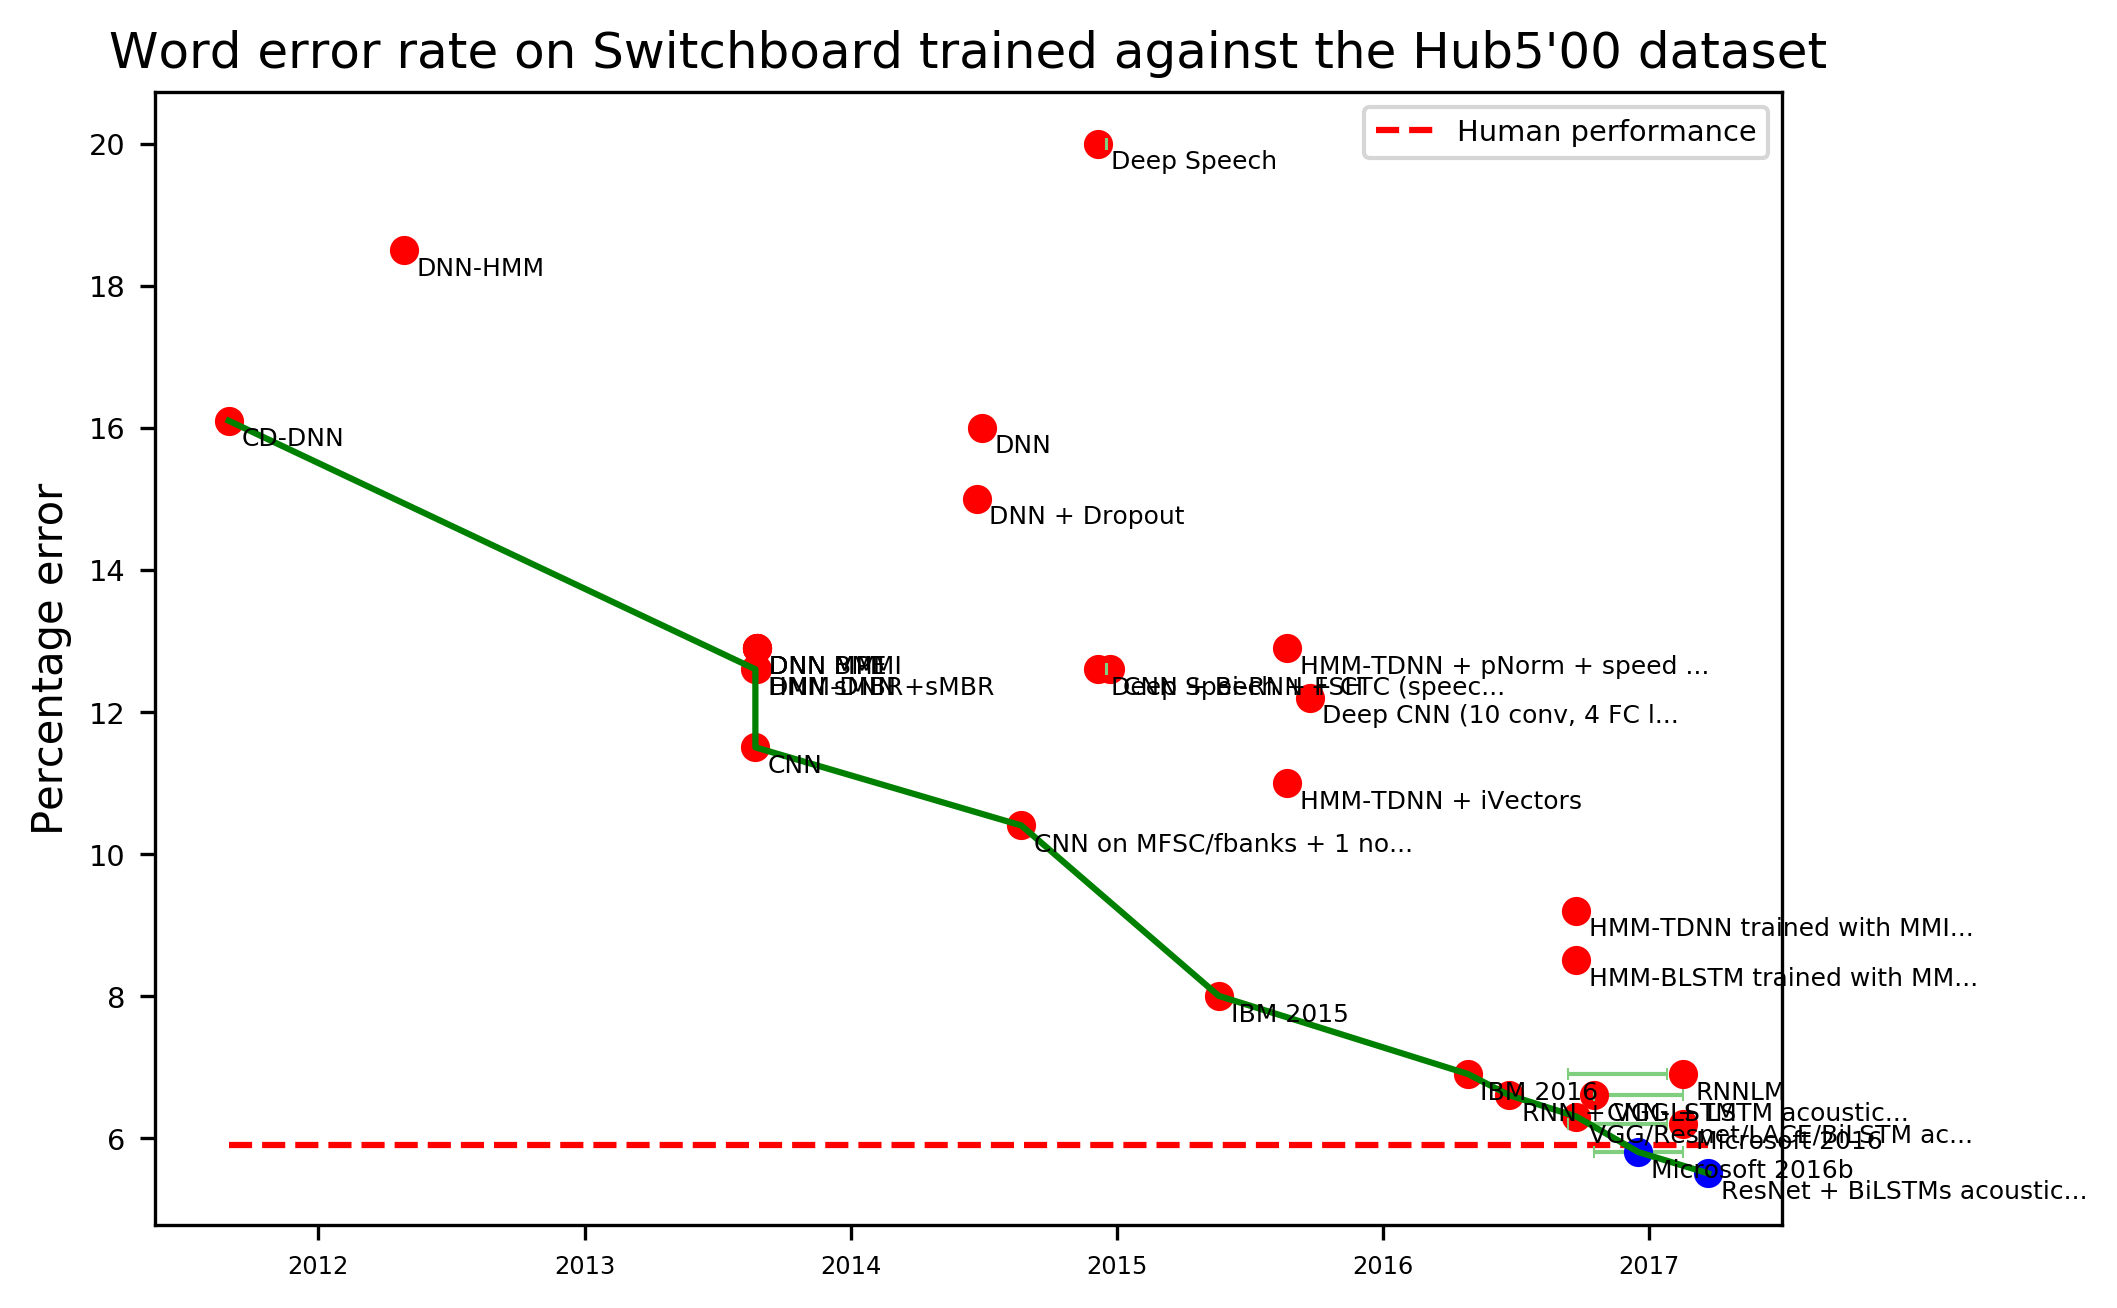
\includegraphics[width=0.5\linewidth]{figures/DL_fundamentals/speech_recog_perf.png}
    %         {\tiny \href{https://www.eff.org/ai/metrics}{Source}}
    %     \end{center}
    % \end{frame}
    
    \subsection[DL history]{From the artificial neuron to deep learning}
    \begin{frame}{\secname}{\subsecname}
        \begin{center}
            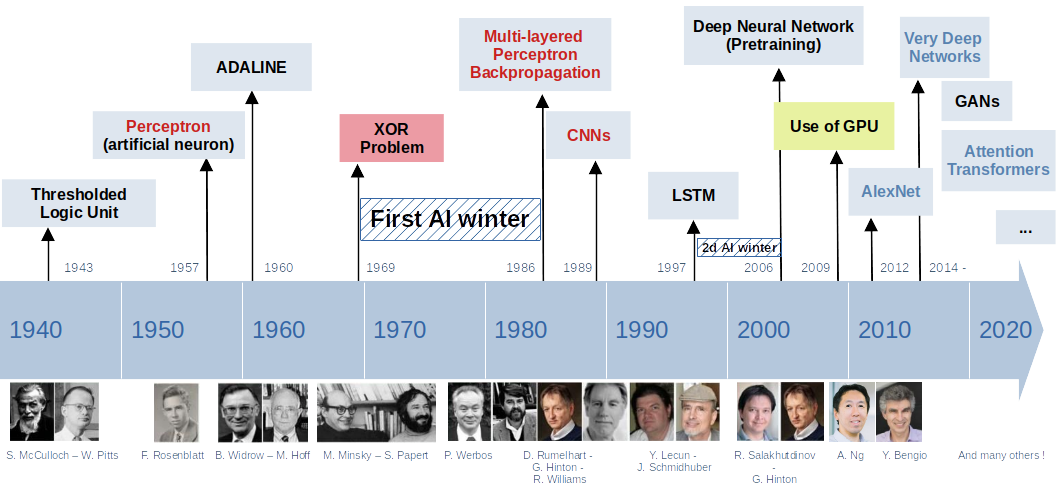
\includegraphics[width=\linewidth]{figures/DL_fundamentals/DL_history_mik.png}
        \end{center}
    \end{frame}
    
    \begin{frame}{\secname}{\subsecname}
        % ML concepts to end up with the specificity of DL
        \sout{Machine} learning principle
        
        \alert{Deep}
        \begin{center}
            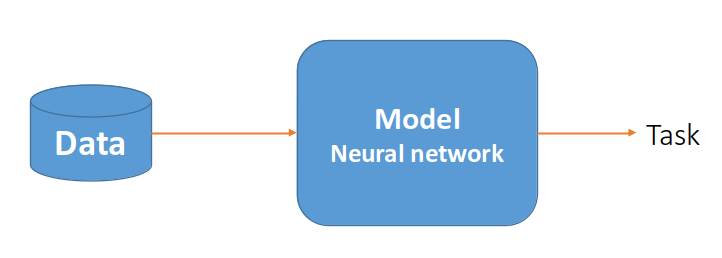
\includegraphics[width=0.82\linewidth]{figures/Context/DL_principle.png}
        \end{center}
        \begin{itemize}
            \item The features are learned by the model
            \item Search for regularity with an over-parametrized model within large sets of data
        \end{itemize}
    \end{frame}
    
    \subsection[Building a NN]{Building a neural network }
    \begin{frame}{\secname}{\subsecname}
        The artificial neuron, or \alert{perceptron}, is the fundamental component of neural networks
        \begin{center}
            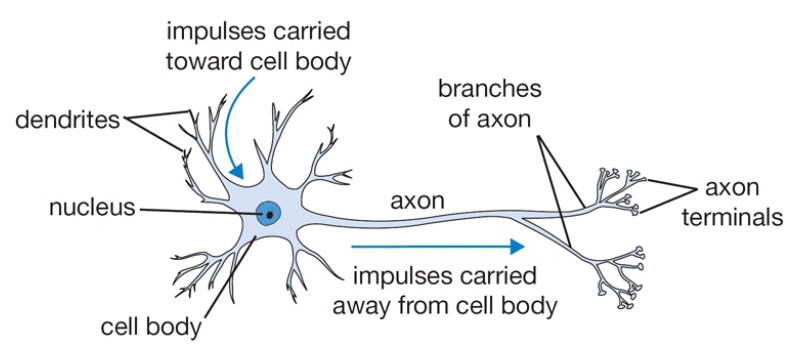
\includegraphics[width=0.48\linewidth]{figures/DL_fundamentals/biological_neuron2.png}%
            \hspace{0.08\linewidth}
            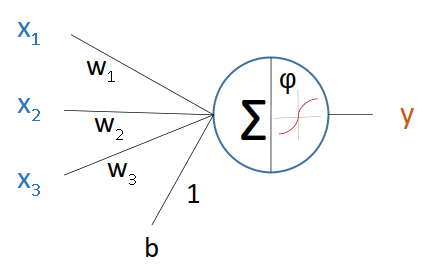
\includegraphics[width=0.4\linewidth]{figures/DL_fundamentals/artificial_neuron.png}
        \end{center}

        \begin{itemize}
            \item Inspired from the biological neuron
            \item Simple mathematical operation followed by a non-linear \alert{activation function}: $y=\varphi(\sum_i w_i \cdot x_i + b)$
            \item Learning ability comes from the trainable \alert{parameters} $w_i$ and $b$, also named \alert{weights}
        \end{itemize}
    \end{frame}
    \begin{frame}{\secname}{\subsecname}
        There exists a large variety of activation functions. Some popular ones:
        \begin{center}
            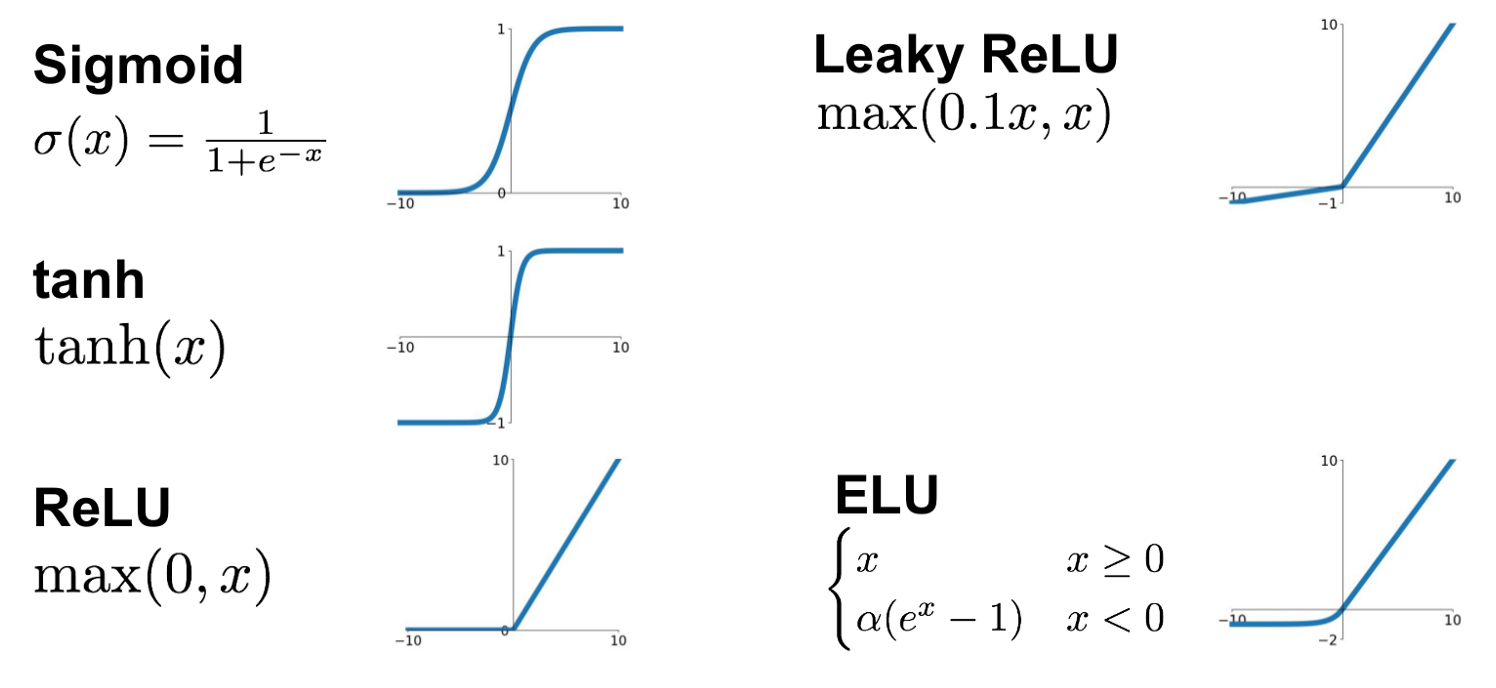
\includegraphics[width=0.9\linewidth]{figures/DL_fundamentals/activation-func.png}
        \end{center}
        \vspace{-1em}
        \begin{itemize}
            \item Sigmoid and tanh are \textit{historical} activation functions but they saturate $\rightarrow$ vanishing gradient
            \item ReLU and its derivatives solve the vanishing gradient issue
        \end{itemize}
    \end{frame}
    \begin{frame}{\secname}{\subsecname}
        Neural networks are orgnized as layers of neurons:
        \vspace{-0.8em}
        \begin{center}
            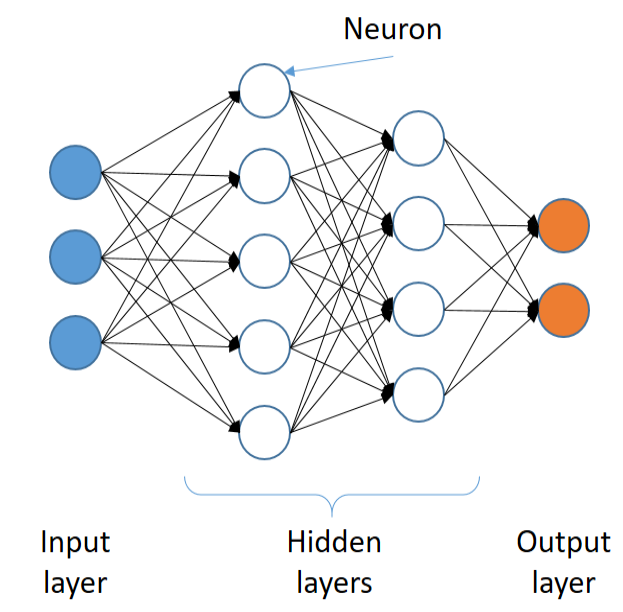
\includegraphics[width=0.45\linewidth]{figures/DL_fundamentals/artificial_neural_network.png}
        \end{center}
        \vspace{-1em}
        \begin{itemize}
            \item This kind of neural network is a \alert{multilayer perceptron} composed of \alert{fully connected layers}
            \item Deep learning $\rightarrow$ 3 \alert{hidden layers} or more
        \end{itemize}
    \end{frame}
    
    \subsection[Training a NN]{Training a neural network }
    \begin{frame}{\secname}{\subsecname}
        The training process
        \begin{enumerate}
            \item Collect and prepare the training data
            \item Train the model with all the data $\rightarrow$ 1 \alert{epoch}
            \item Evaluate the model performance
            \item If necessary, repeat steps 2 and 3
        \end{enumerate}
        \vspace{-0.7em}
        \begin{center}
            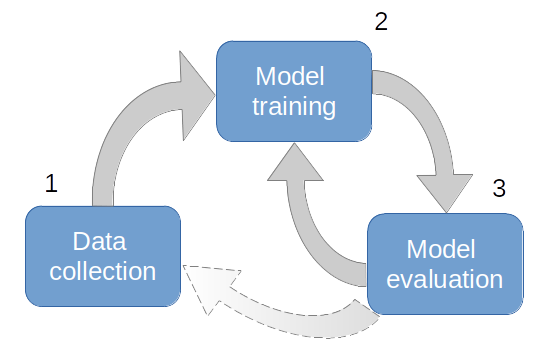
\includegraphics[width=0.45\linewidth]{figures/DL_fundamentals/DL_training_process_epoch.png}
        \end{center}
        \vspace{-0.7em}
        \begin{itemize}
            \item Neural networks generally require from \textbf{tens to hundreds epochs}
        \end{itemize}
    \end{frame}
    \begin{frame}{\secname}{\subsecname}
        Going into the details of step 2 (model training)
        \begin{itemize}
            \item Data generally don't fit in memory $\rightarrow$ \alert{batch} of data
            \item Training the model with a batch is an \alert{iteration}
            \item The iteration process:
            \begin{enumerate}
                \item Neural network forward pass = prediction on the batch
                \item Evaluate the prediction error
                \item Update neural networks weights to minimize the prediction error (backward pass)
            \end{enumerate}
            \item We repeat this process until all the data are consumed\\
            $\rightarrow N_{iteration} = \frac{N_{data}}{N_{batch}} \approx hundreds \rightarrow thousands$
        \end{itemize}
        \vspace{-0.7em}
        \begin{center}
            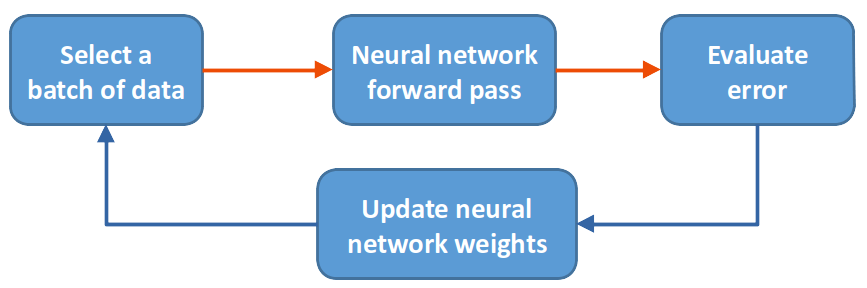
\includegraphics[width=0.7\linewidth]{figures/DL_fundamentals/DL_training_process_iteration.png}
        \end{center}
    \end{frame}
    \begin{frame}{\secname}{\subsecname}
        Going into more details
        \begin{itemize}
            \item We evaluate the error with a \alert{loss} function
            \item For supervised learning
            \begin{itemize}
            	\item Classification: Cross-Entropy (Softmax + NLL) \\
            	\vspace{0.5em}
            	$L = \frac{1}{n} \sum_n \sum_i -y_{true, i} \cdot \log(p(c_i=1| x))$ with $p(c_i=1| x) = \frac{\exp^{y_{pred,i}}}{\sum_j \exp^{y_{pred,j}}}$ and $y_{true} = [\overset{1}{0} 0 \dots 0 \overset{i}{1} 0\dots \overset{c}{0}]$
            	\vspace{0.5em}
            	\item Regression: MSE\\ 
            	\vspace{0.5em}
            	$L = \frac{1}{n}\sum_n (y_{pred}-y_{true})^2$
            \end{itemize}
        \end{itemize}
        \begin{center}
            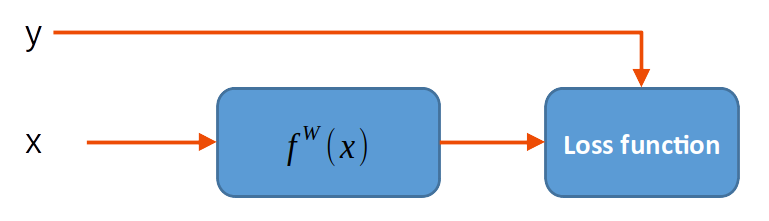
\includegraphics[width=0.78\linewidth]{figures/DL_fundamentals/DL_training_process_detail.png}
        \end{center}
    \end{frame}
	\begin{frame}{\secname}{\subsecname}
		\begin{itemize}
			\item We update the weights to minimize the loss
			\item Stochastic Gradient Descent (\alert{SGD}) $\rightarrow$ \alert{optimizer}
			\item $W_{t+1} = W_t - \eta \cdot \nabla_{W_t}L$ with $\eta$ the \alert{learning rate}
		\end{itemize}
		\begin{columns}
			\begin{column}{0.7\textwidth}
				\begin{itemize}
					\item Challenges
					\begin{itemize} 
					    \item Finding a "good" local minimum
					    \item Choosing the lr is difficult
					    \item The initial lr might not be optimal during the whole training process
					    \item The same lr might not be optimal for all the parameters
					    \item Avoiding saddle point is crucial
					\end{itemize}
				\end{itemize}
			\end{column}
			\begin{column}{0.3\textwidth}
				\begin{center}
					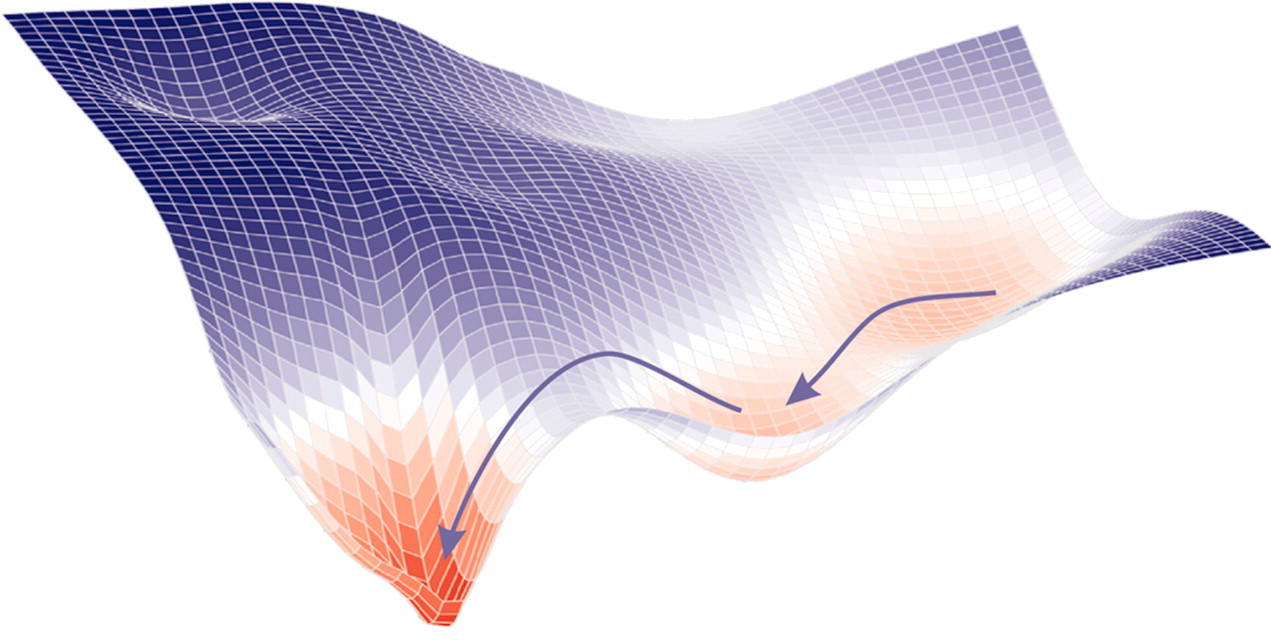
\includegraphics[width=\linewidth]{figures/DL_fundamentals/gradient_descent.png}
				\end{center}
			\end{column}
		\end{columns}
		\begin{itemize}
		    \item Several evolutions: momentum, adative methods including \alert{Adam} \dots
			\item See \cite{Ruder2016} for details 
		\end{itemize}
	\end{frame}   
	\begin{frame}{\secname}{\subsecname}
	    \begin{itemize}
	        \item But how can we apply SGD to \textbf{millions} of parameters ?
	        \item Solving analytically $\nabla_{W_t}L$ is untractable
	        \item Solution: the \alert{backpropagation} algorithm !
	    \end{itemize}
	    \begin{example}
	        Consider the following neural network:
	        \begin{center}
				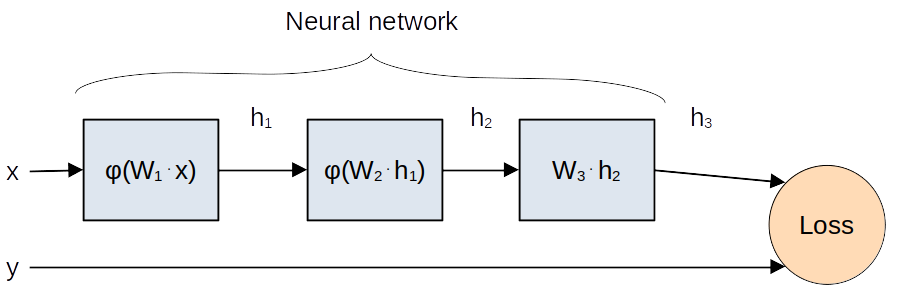
\includegraphics[width=0.8\linewidth]{figures/DL_fundamentals/backpropagation_mik.png}
			\end{center}
			\vspace{-0.7em}
			with $\varphi(a) = max(0, a)$ and a Cross-entropy loss
	    \end{example}
    \end{frame}
    \begin{frame}{\secname}{\subsecname}
        \vspace{-1.5em}
	    \begin{exampleblock}{}
	        For gradient descent, we need to compute $\frac{\partial L}{\partial W_1}$, $\frac{\partial L}{\partial W_2}$ and $\frac{\partial L}{\partial W_3}$
	        
			The gradient of the loss w.r.t. the last features $h_3$ is:
			\begin{itemize}
			    \item $\frac{\partial L}{\partial h_3} = p(c|x) - y_{true}$
			\end{itemize}
			Then, with the chain rule, we can compute:
			\begin{itemize}
			    \item $\frac{\partial L}{\partial W_3} =\frac{\partial L}{\partial h_3}\frac{\partial h_3}{\partial W_3} = (p(c|x)-y_{true})\cdot h_2^T$
			    \item $\frac{\partial L}{\partial W_2} =\frac{\partial L}{\partial h_2}\frac{\partial h_2}{\partial W_2} = \frac{\partial L}{\partial h_3}\frac{\partial h_3}{\partial h_2}\frac{\partial h_2}{\partial W_2}$
			    \item $\frac{\partial L}{\partial W_1} =\frac{\partial L}{\partial h_1}\frac{\partial h_1}{\partial W_1} = \frac{\partial L}{\partial h_2}\frac{\partial h_2}{\partial h_1}\frac{\partial h_1}{\partial W_1}$
			\end{itemize}
			\begin{center}
				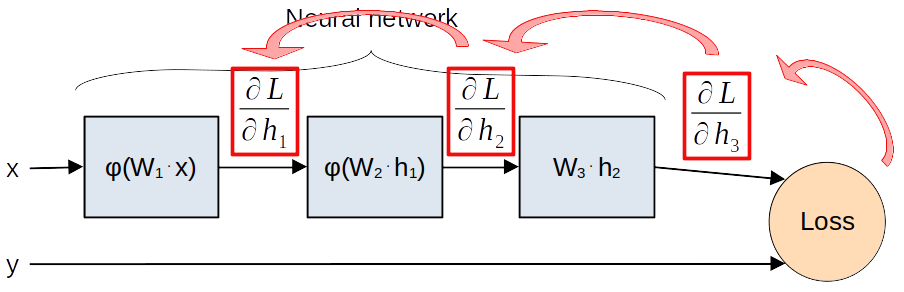
\includegraphics[width=0.7\linewidth]{figures/DL_fundamentals/backpropagation_mik_grad.png}
			\end{center}
			\vspace{-0.5em}
         \end{exampleblock}
    \end{frame}
    \begin{frame}{\secname}{\subsecname}
        Vocabulary break
        \begin{itemize}
            \item The \alert{parameters} are the trainable weights of the network
            \item The \alert{hyperparameters} are defined by the expert to set up the experiment, including:
            \begin{itemize}
                \item The network definition (number, size and type of each layer)
                \item The choice of the optimizer (SGD, Adam \dots)
                \item The learning rate and its evolution during the training
                \item The loss function
                \item \dots
            \end{itemize}
        \end{itemize}
    \end{frame}
    \subsection{Ressources needed}
    \begin{frame}{\secname}{\subsecname}
        We are able to design and train neural networks to do fancy stuff, but:
        \begin{itemize}
            \item Neural networks can have millions of parameters (the heaviest architecture has currently 1.6 trillion !!)
            \item The training process implies thousands of iterations and tens to hundreds epochs
            \item The hyperparameter space is huge !
        \end{itemize}
        \vspace{1em}
        $\rightarrow$ We need efficient computing ressources
    \end{frame}
    \begin{frame}{\secname}{\subsecname}
        Fortunately, most DL computations can be carried out in parallel\\
        $\rightarrow$ we can benefit from GPUs (A. Ng et al., 2009)
        \begin{itemize}
            \item GPUs are part of the success of neural networks
            \item The training time is divided by up to 70 compared to CPU
            \item Modern GPUs are composed of thousands of processing units, some specialized in DL operations (e.g., Tensorcores)
            \item NVIDIA CUDA (+ cuDNN) drivers contain very optimized algorithms for DL fundamental operations (matrix multipication, convolution\dots)
        \end{itemize}
    \end{frame}
    \begin{frame}{\secname}{\subsecname}
        We also need highly efficient software libraries:
        \begin{itemize}
            \item To efficiently exploit hardware capabilities
            \item To offer high level abstraction to deep learning components
            \item To take care of the computation graph and gradient operations
            \item To manage engineering code and focus on research (hyperparameter definition)
        \end{itemize}
    \end{frame}
    \begin{frame}{\secname}{\subsecname}
        General deep learning stack
        \begin{center}
            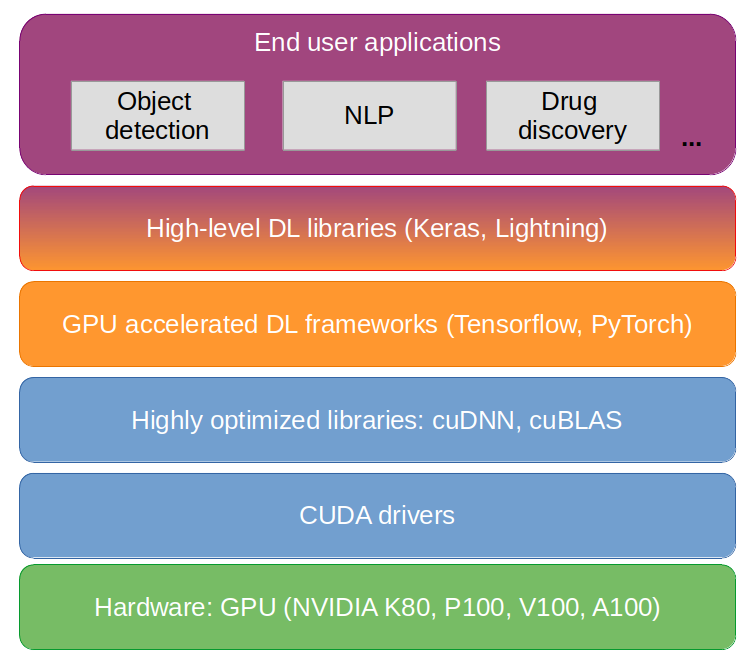
\includegraphics[width=0.7\linewidth]{figures/DL_fundamentals/DL_stack.png}
        \end{center}
    \end{frame}
    % \subsection[NN regularization]{Neural network regularization}
    % \begin{frame}{\secname}{\subsecname}
    %     \begin{itemize}
    %         \item NN can overfit, we may need to regularize the model during training
    %         \item Dropout
    %         \item Batchnorm
    %         \item Loss penalty: L1 (lasso), L2, gradient-based
    %     \end{itemize}
    % \end{frame}
    
    \subsection[DL libraries]{Deep learning libraries}
    \begin{frame}{\secname}{\subsecname}
        There exists many DL frameworks
        \begin{itemize}
            \item The elder ones: Caffe, Theano, Torch
            \item The outsiders: Chainer, Deeplearning4j, MXNet, Caffe2
            \item The leaders: 
            \begin{itemize}
                \item Tensorflow (static graph) \href{https://www.tensorflow.org/}{\raisebox{-.3\height}{
\includegraphics[width=0.12\linewidth]{figures/DL_fundamentals/tensorflow_logo.png}}}
                \item \textbf{PyTorch} (dynamic graph) \href{https://pytorch.org}{\raisebox{-.3\height}{
\includegraphics[width=0.08\linewidth]{figures/DL_fundamentals/pytorch-logo.png}}}
            \end{itemize}
        \end{itemize}
        They offer interfaces in several languages: \textbf{Python}, C++, Java, Javascript
    \end{frame}
    
    \begin{frame}{\secname}{\subsecname}
        PyTorch
        \begin{center}
            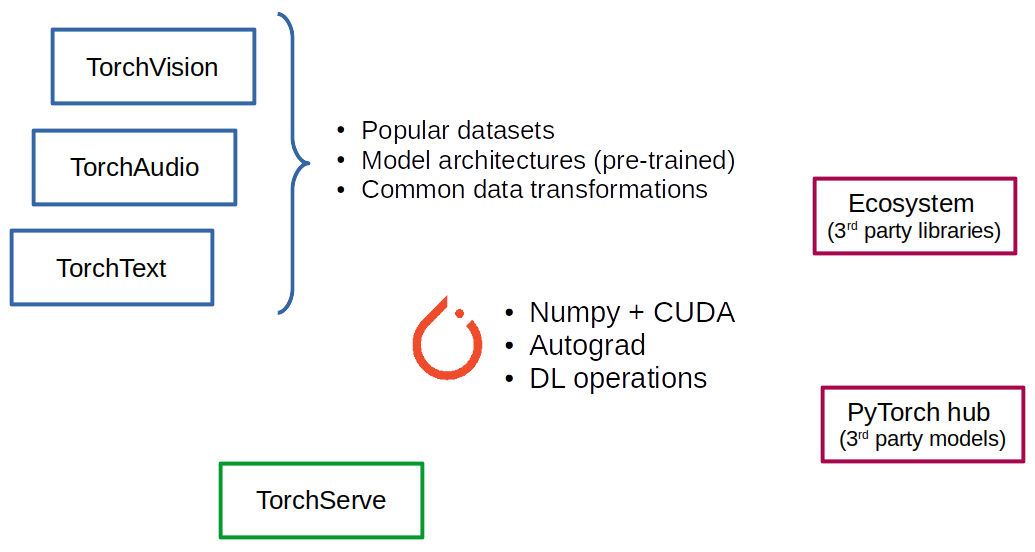
\includegraphics[width=\linewidth]{figures/DL_fundamentals/Pytorch_ecosystem.png}
        \end{center}
    \end{frame}
    \begin{frame}[fragile]{\secname}{\subsecname}
        PyTorch quickstart
        \begin{itemize}
            \item Basic data structure: PyTorch tensor $\rightarrow$ Numpy array + CUDA + autograd
            \begin{minted}{python}
import torch
import numpy as np

np_array = np.array([0, 1, 2])
torch_tensor = torch.from_numpy(np_array)
torch_tensor
> tensor([0, 1, 2])
torch_tensor.requires_grad
> False
            \end{minted}
            \item By default, tensors \textbf{do not} retain gradient information
        \end{itemize}
    \end{frame}
    \begin{frame}[fragile]{\secname}{\subsecname}
        Working with data
        \begin{itemize}
            \item Standard vision datasets can be loaded from TorchVision
            \begin{minted}{python}
from torchvision.datasets import CIFAR10
from torchvision.transforms import ToTensor

dataset = CIFAR10(root='./data', train=True, 
                  download=True, 
                  transform=ToTensor())
            \end{minted}
            \item The output of torchvision datasets are PILImage images
            \item We need to transform them to Tensors
            \item We can implement custom datasets by inheriting Dataset class
        \end{itemize}
    \end{frame}
    \begin{frame}[fragile]{\secname}{\subsecname}
        Working with data
        \begin{itemize}
            \item DataLoader takes care of sampling data batches during training
            \begin{minted}{python}
from torch.utils.data import DataLoader
training_data = DataLoader(dataset, 
                           batch_size=32, 
                           num_workers=4, 
                           shuffle=True)
            \end{minted}
        \end{itemize}
    \end{frame}
    \begin{frame}[fragile]{\secname}{\subsecname}
        Creating neural networks
        \begin{itemize}
            \item We find neural network layers in torch.nn
            \begin{minted}{python}
from torch import nn
nn.Linear(in_features=512, out_features=512)
nn.ReLU()
nn.Conv2d(in_channels=3, out_channels=16, 
          kernel_size=3, padding=1)
            \end{minted}
            \item We can build simple models as Sequential
            \begin{minted}{python}
model = nn.Sequential(
    nn.Linear(in_features=32, out_features=16),
    nn.LeakyReLU(),
    nn.Linear(in_features=16, out_features=10)
)
            \end{minted}
        \end{itemize}
    \end{frame}
    \begin{frame}[fragile]{\secname}{\subsecname}
        \begin{itemize}
            \item For more complex models
            \begin{minted}{python}
class NeuralNetwork(nn.Module):
    def __init__(self):
        super(NeuralNetwork, self).__init__()
        self.flatten = nn.Flatten()
        self.linear_relu_stack = nn.Sequential(
            nn.Linear(28*28, 512),
            nn.ReLU(),
            nn.Linear(512, 10),
        )

    def forward(self, x):
        x = self.flatten(x)
        logits = self.linear_relu_stack(x)
        return logits
            \end{minted}
        \end{itemize}
    \end{frame}
    
    % \subsection[Key notions]{Key notions}
    % \begin{frame}{\secname}{\subsecname}
    %     The following is very important !
    % \end{frame}
    
    \subsection[Hands on]{First hands on session}
    \begin{frame}{\secname}{\subsecname}
        \begin{center}
            Time to work !
        \end{center}
        3 tutorials to smoothly enter the deep learning world:
        \begin{itemize}
            \item T1: Fitting a noisy sinusoid with a MLP
            \item T2: Training a MLP on a binary classification case
            \item T3: Training a MLP on a multi-class classification case
        \end{itemize}
    \end{frame}


%----------------------------------------------------------------------------
\section[Going deep]{Part II, Going (really) deep}
    
    \begin{frame}{\secname}
        Part II outline
        \begin{itemize}
            \item Convolutional neural network: overcoming the limitations of MLP
            \item Famous very deep networks and modern architectures
            \item Transfer learning: recycling knowledge
            % \item Introduction to explainability
            \item High-level deep learning library and logging tool
        \end{itemize}
    \end{frame}
    
    \subsection{Convolutional neural networks}
    \begin{frame}{\secname}{\subsecname}
        The MLP is a universal function approximator \cite{cybenko1989approximation}, but:
        \begin{itemize}
            \item The number of parameters can rapidly grow with the size of the input and the number of layers $\rightarrow N_i = (n_{i-1}+1) \times n_i$
            \begin{example}
                CIFAR10 dataset: 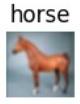
\includegraphics[width=0.8cm]{figures/DL_fundamentals/CIFAR10-horse.png}\\
                \begin{itemize}
                    \item Small RGB images of 32x32 pixels
                    \item Fully connected $\rightarrow$ each pixel is a feature
                    \item \textbf{Each neuron} of the first hidden layer would have 32x32x3 + 1 = {\color{orange}3073 parameters} !
                \end{itemize}
            \end{example}
        \end{itemize}
    \end{frame}
    \begin{frame}{\secname}{\subsecname}
        \begin{itemize}
            \item MLP is not translation invariant $\rightarrow$ severe drawback for computer vision
        \end{itemize}
        \begin{columns}
            \begin{column}{0.5\textwidth}
               The {\color{orange} orange weights} are modified to better recognize Homer
            \end{column}
            \begin{column}{0.5\textwidth}
                \begin{center}
                 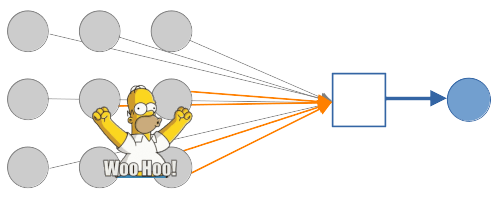
\includegraphics[width=0.9\textwidth]{figures/DL_fundamentals/MLP_invariance_issue_homer_down.png}
                 \end{center}
            \end{column}
        \end{columns}
        \begin{columns}
            \begin{column}{0.5\textwidth}
               The {\color{ForestGreen}green weights} are modified to better recognize Homer
            \end{column}
            \begin{column}{0.5\textwidth}
                \begin{center}
                 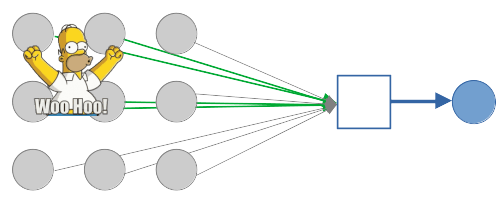
\includegraphics[width=0.9\textwidth]{figures/DL_fundamentals/MLP_invariance_issue_homer_up.png}
                 \end{center}
            \end{column}
        \end{columns}
        \vspace{0.8em}
        $\rightarrow$ Learning redundant features + not robust
    \end{frame}
    \begin{frame}{\secname}{\subsecname}
        In images,
        \begin{columns}
            \begin{column}{0.5\textwidth}
               \begin{itemize}
                   \item Nearby pixels are more strongly related than distant ones
                   \item Objects are built up out of small parts
               \end{itemize}
            \end{column}
            \begin{column}{0.5\textwidth}
                \begin{center}
                 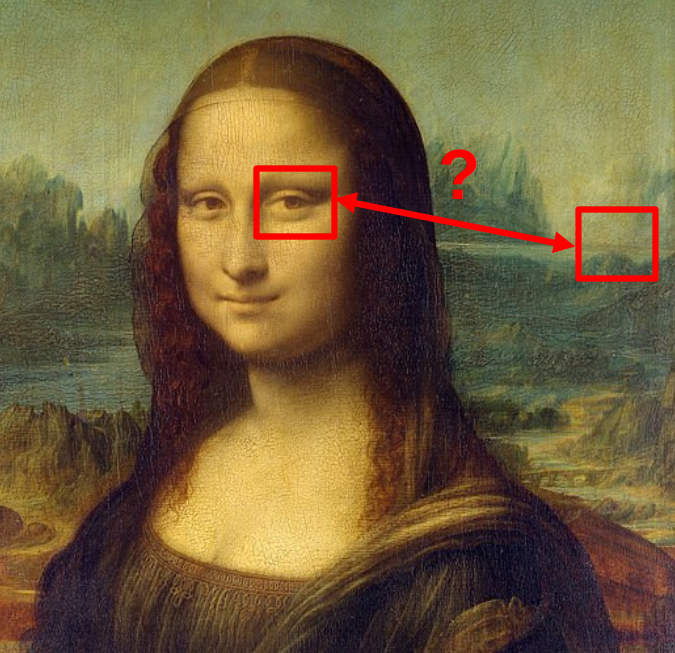
\includegraphics[width=0.6\textwidth]{figures/DL_fundamentals/mona_lisa.png}
                 \end{center}
            \end{column}
        \end{columns}
        \vspace{1em}
        Translates to other fields, e.g., text analysis:\\ 
        {\tiny Towns and {\color{orange}cities} across {\color{orange}Scotland} would be devastated if the country’s coastline was hit by a tsunami of the kind that happened 8,200 years ago, according to an academics’ study.
        While about 370 miles of Scotland’s northern and eastern coastline were affected when the Storegga tsunami struck, the study suggests a modern-day disaster of the same {\color{ForestGreen}magnitude} would have worse consequences. (source: The Guardian)}
    \end{frame}
    \begin{frame}{\secname}{\subsecname}
    Solution: the convolution (derives from the visual cortex)
        \begin{itemize}
            % \item Derives from the visual cortex of mamals
            \item The convolutional neuron operates on a local neighborhood $\rightarrow$ shared weights = convolution \alert{kernel}
            \item The kernel slides over the input with a chosen \alert{stride}\\ $\rightarrow$ 1 position = 1 pixel of the output \alert{feature map}
            \item 1 convolutional neuron $\rightarrow$ 1 output feature map
            \item Convolution layer = stack of \textit{n} neurons $\rightarrow$ \textit{n} feature maps
        \end{itemize}
        \vspace{-1em}
        \begin{center}
            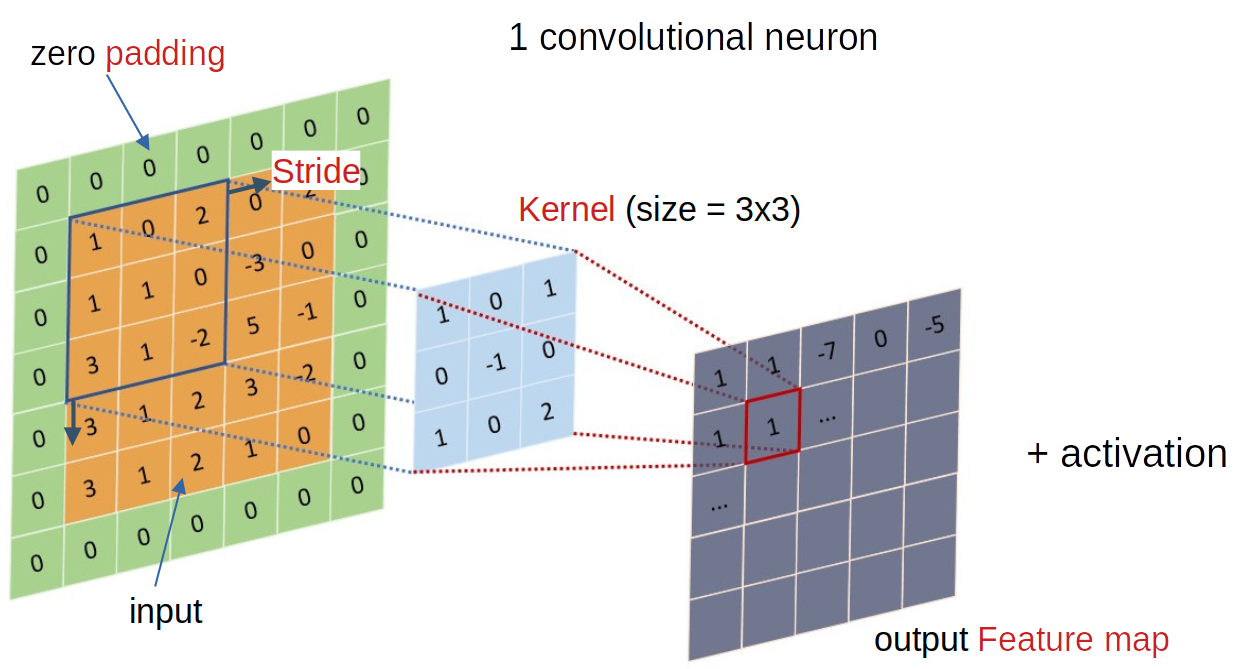
\includegraphics[width=0.7\linewidth]{figures/DL_fundamentals/convolution.png}
        \end{center}
    \end{frame}
    \begin{frame}{\secname}{\subsecname}
        The \alert{pooling} operation
        \begin{itemize}
            \item Also operates on a local neighborhood
            \item A form of non-linear down-sampling (with stride $>$ 1)
            \item Participates to (local) spatial invariance
            \item Standard pooling functions: max, average or convolution
        \end{itemize}
        \vspace{-1em}
        \begin{center}
            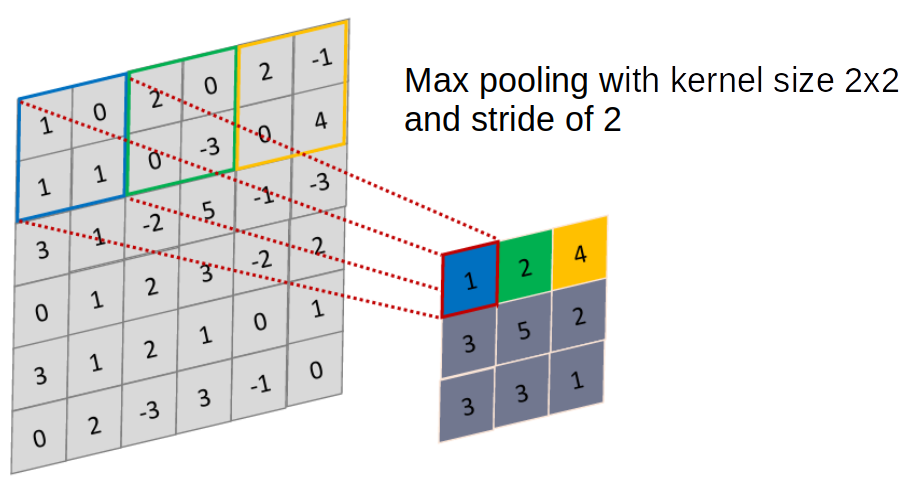
\includegraphics[width=0.7\linewidth]{figures/DL_fundamentals/maxpooling.png}
        \end{center}
    \end{frame}
    \begin{frame}{\secname}{\subsecname}
        Building a convolutional neural network (\alert{CNN})
        \begin{itemize}
            \item CNN = encoder + decoder
            \item Encoder
            \begin{itemize}
                \item Learns a (compressed) latent representation of the data
                \item A lasagna of convolution layers (including activations) and pooling layers
            \end{itemize}
            \item Decoder
            \begin{itemize}
                \item Learns to solve the task from the latent representation
                \item One or more fully connected layers
            \end{itemize}
            \item Advantages of CNN over MLP
            \begin{itemize}
                \item The total number of parameters is dramatically reduced
                \item Translation invariance
                \item Pixel position and neighborhood have semantic meanings
            \end{itemize}
        \end{itemize}
    \end{frame}
    \begin{frame}{\secname}{\subsecname}
        Example: \href{http://yann.lecun.com/exdb/lenet/}{LeNet-5} for character recognition (1998)
        \begin{center}
            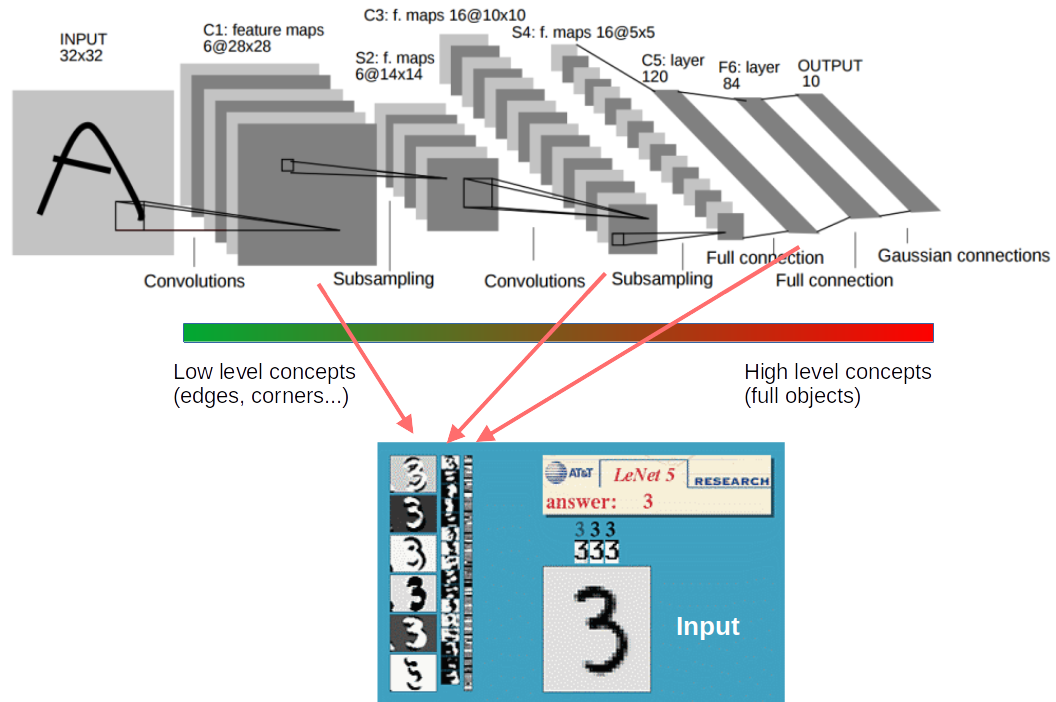
\includegraphics[width=0.95\linewidth]{figures/DL_fundamentals/LeNet5.png}
        \end{center}
    \end{frame}

    \subsection[Famous DL architectures]{Famous deep learning architectures}
    \begin{frame}{\secname}{\subsecname}
        \textbf{AlexNet}, the pioneer: beating standard CV methods in the ImageNet Large Scale Visual Recognition Challenge 2012 \cite{krizhevsky2012imagenet}
        \vspace{-0.8em}
        \begin{center}
            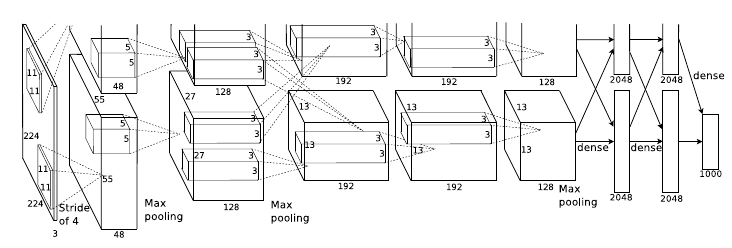
\includegraphics[width=0.95\linewidth]{figures/Going_deeper/Alexnet.png}
        \end{center}
        \vspace{-1em}
        \begin{columns}
            \begin{column}{0.4\textwidth}
                \begin{itemize}
                    \item 5 convolution layers
                    \item ReLU activations
                    \item Dropout
                \end{itemize}
            \end{column}
            \begin{column}{0.6\textwidth}
                \begin{itemize}
                    \item Multi-GPUs training
                    \item Top-5 error: 15.3\% vs 26.1\%
                \end{itemize}
            \end{column}
        \end{columns}
    \end{frame}
    \begin{frame}{\secname}{\subsecname}
        \vspace{-1em}
        \begin{columns}
            \begin{column}{0.5\textwidth}
                \begin{center}
                    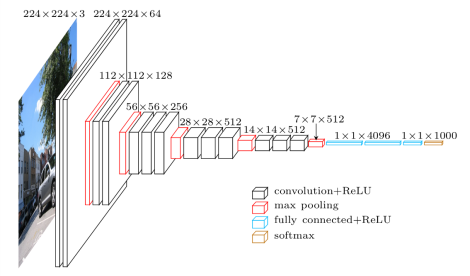
\includegraphics[width=\linewidth]{figures/Going_deeper/vgg16.png}\\ \vspace{-1.5em}{\tiny VGG-16}
                \end{center}
            \end{column}
            \begin{column}{0.5\textwidth}
                \begin{center}
                    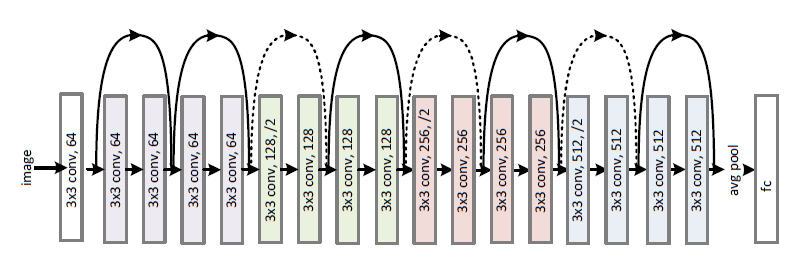
\includegraphics[width=\linewidth]{figures/Going_deeper/resnet18.png} \\ \vspace{-0.8em} {\tiny ResNet-18}
                \end{center}
            \end{column}
        \end{columns}
        \begin{columns}
            \begin{column}{0.7\textwidth}
                \begin{center}
                    \vspace{-0.8em} 
                    \includegraphics[width=\linewidth]{figures/Going_deeper/inception_v1.png}\\ \vspace{-0.8em} {\tiny Inception-V1}
                \end{center}
            \end{column}
            \begin{column}{0.3\textwidth}
                \begin{center}
                    \vspace{-1.8em} 
                    \includegraphics[width=\linewidth]{figures/Going_deeper/transformer.png}\\ \vspace{-0.8em} {\tiny Transformer}
                \end{center}
            \end{column}
        \end{columns}
        \vspace{-2em}
        Hundreds of layers and billions of parameters !
    \end{frame}
    
    % \begin{frame}{\secname}{\subsecname}
    %     \textbf{VGG}, starting to go deep \cite{Simonyan2014vgg}
    %     \vspace{-0.8em}
    %     \begin{center}
    %         \includegraphics[width=0.75\linewidth]{figures/Going_deeper/vgg16.png}{\tiny VGG-16}
    %     \end{center}
    %     \vspace{-1em}
    %     \begin{columns}
    %         \begin{column}{0.5\textwidth}
    %             \begin{itemize}
    %                 \item Up to 19 layers\\ $\rightarrow$ (144 M parameters)
    %                 \item $3\times 3$ convolution kernels
    %             \end{itemize}
    %         \end{column}
    %         \begin{column}{0.5\textwidth}
    %             \begin{itemize}
    %                 \item Group of convolutions followed by max-pooling
    %                 \item Top-5 error on\\ ILSVRC 2012: 6.8\%
    %             \end{itemize}
    %         \end{column}
    %     \end{columns}
    % \end{frame}
    % \begin{frame}{\secname}{\subsecname}
    %     \textbf{ResNet}, going really deep with residual connections \cite{he2016deep,he2016identity}
    %     \vspace{-0.8em}
    %     \begin{center}
    %         \includegraphics[width=0.83\linewidth]{figures/Going_deeper/resnet18.png} {\tiny ResNet-18}
    %     \end{center}
    %     \vspace{-1em}
    %     \begin{columns}
    %         \begin{column}{0.6\textwidth}
    %             \begin{itemize}
    %                 \item Up to 1202 layers !
    %                 \item Too many layers cause gradient vanishing issue\\ $\rightarrow$ Residual connections 
    %                 \item Top-5 error on ILSVRC 2012: 4.8\% (ResNet-200)
    %             \end{itemize}
    %         \end{column}
    %         \begin{column}{0.4\textwidth}
    %             \begin{center}
    %                 \includegraphics[width=\linewidth]{figures/Going_deeper/residual_block.png}
    %             \end{center}
    %         \end{column}
    %     \end{columns}
    % \end{frame}
    % \begin{frame}{\secname}{\subsecname}
    %     \textbf{Inception}, going deep and wide
    %     \cite{szegedy2015going,Szegedy_2016_CVPR_rethinking}
    %     \vspace{-0.8em}
    %     \begin{center}
    %         \includegraphics[width=\linewidth]{figures/Going_deeper/inception_v1.png}\\ \vspace{-0.8em} {\tiny Inception-V1}
    %     \end{center}
    %     \vspace{-1em}
    %     \begin{columns}
    %         \begin{column}{0.6\textwidth}
    %             \begin{itemize}
    %                 \item Multiple-size filters on the same level
    %                 \item 42 layers (V3) but faster than VGG 
    %                 \item Top-5 error on ILSVRC 2012: 4.2\% (Inception-V3)
    %             \end{itemize}
    %         \end{column}
    %         \begin{column}{0.4\textwidth}
    %             \begin{center}
    %                 \includegraphics[width=0.85\linewidth]{figures/Going_deeper/inception_module.png}\\\vspace{-0.8em}{\tiny Inception-V3 module}
    %             \end{center}
    %         \end{column}
    %     \end{columns}
    % \end{frame}
    % \begin{frame}{\secname}{\subsecname}
    %     \textbf{Attention} is all you need !
    %     \begin{itemize}
    %         \item Helps the model focus on relevant features
    %         \item Originates in NLP: main component of Transformer architecture \cite{vaswani2017attention, devlin2019bert} $\rightarrow$ SOTA in neural machine translation and image captioning
    %         \item Increasing use in computer vision architectures
    %         \item Standalone or in combination with convolution block (e.g., ResNet-SE \cite{hu2018squeeze})
    %         \item Attention types in CV
    %         \begin{itemize}
    %             \item pixel-wise attention, also named spatial attention
    %             \item channel-wise attention
    %             \item combination of both
    %         \end{itemize}
    %     \end{itemize}
            
    % \end{frame}
    % \begin{frame}{\secname}{\subsecname}
    %     Dual Attention \cite{sun2020saunet} example
    %     \vspace{-0.8em}
    %     \begin{center}
    %         \includegraphics[width=\linewidth]{figures/Going_deeper/dual_attention.png}\\\vspace{-0.8em}
    %     \end{center}
    % \end{frame}

    \subsection{Transfer learning}
    \begin{frame}{\secname}{\subsecname}
        Training modern DL architectures from scratch for a specific application is costly. It requires:
        \begin{itemize}
            \item Huge amount of data
            \item Powerful GPUs
            \item Time to tweak the hyperparameters
        \end{itemize}
        \vspace{-0.8em}
        \begin{alertblock}{}
            Training the Transformer \cite{vaswani2017attention} for NLP, including architecture search, has emitted 284 tonnes of $CO_2$ ! \cite{strubell2019energy} 
        \end{alertblock}

        Then, let's try to recycle with \textbf{transfer learning} !
        \begin{itemize}
            \item Many SOTA algorithms trained on standard data sets are available !
            \item We can continue the training on our (similar) specific task (and our little data)
            
            $\rightarrow$ Leveraging previously learned features
        \end{itemize}
    \end{frame}
    \begin{frame}{\secname}{\subsecname}
        Transfer learning steps
        \begin{enumerate}
            \item Select a model trained on a task similar to your problem
            \item Load layers from trained model
            \item Freeze most of them (generally the first ones) to keep knowledge
            \item Add / change layers to match your task
            \item Train the new and unfrozen layers
        \end{enumerate}
    \end{frame}
    \begin{frame}{\secname}{\subsecname}
        Transfer learning example
        \begin{itemize}
            \item Task: classify between screws and nuts ($\sim$ 500 images)
            \item Model: ResNet-18 trained on ImageNet (1000 classes)
            \item Transfer learning
            \begin{enumerate}
                \item Freeze all the convolutional layers
                \item Replace the last FC layer to match our 2 classes task
                \item Train this last layer on our little data set of screws and nuts
            \end{enumerate}
        \end{itemize}
        \vspace{-1em}
        \begin{center}
            \includegraphics[width=0.82\linewidth]{figures/Going_deeper/transfer_learning.pdf}\\\vspace{-0.8em}
        \end{center}
    \end{frame}
    
    % \subsection[Intro to explainability]{Introduction to explainability}
    % \begin{frame}{\secname}{\subsecname}
    %     Deep learning models are used in several fields with high impact on our lives:
    %     \begin{itemize}
    %         \item Healthcare
    %         \item Insurance
    %         \item Autonomous vehicles
    %         \item Forensics
    %         \item Candidate selection for jobs
    %         \item \dots
    %     \end{itemize}
    %     We need to understand the model's decision !
    %     \begin{itemize}
    %         \item Interpretability: how a drift in the data affects the decision
    %         \item Explainability: better understand the internal mechanics that leads to the decision
    %     \end{itemize}
    % \end{frame}
    % \begin{frame}{\secname}{\subsecname}
    %     Explainable deep learning is a highly active research domain \cite{xie2020explainable}.\\
    %     3 types of method:
    %     \begin{itemize}
    %         \item Model distillation: develop a separate explainable model (such as random forests) that mimic the behavior of the neural network
    %         \item Intrinsic methods: make use specific layers such as attention layers
    %         \item Visualization methods: highlight the most important pixels for model's decision
    %         \begin{itemize}
    %             \item Perturbation-based: comparison of network decision between an input and an altered copy of the input
    %             \item Gradient-based (or backpropagation-based)
    %         \end{itemize}
    %     \end{itemize}
    % \end{frame}
    % \begin{frame}{\secname}{\subsecname}
    %     Gradient-based visual method example: Grad-CAM \cite{selvaraju2017grad}
    %     \vspace{-1em}
    %     \begin{center}
    %         \includegraphics[width=\linewidth]{figures/Going_deeper/grad-cam.pdf}\\\vspace{-0.8em}
    %     \end{center}
    %     \begin{enumerate}
    %         \item Compute the gradient of the output of interest (e.g., 'Tiger Cat') w.r.t. the convolutional feature maps (A)
    %         \item Average each gradient map to obtain a coefficient
    %         \item Sum the feature maps A weighted by their respective coefficient
    %         \item Apply ReLU activation to only keep positive values
    %     \end{enumerate}
    % \end{frame}
    
    \subsection[DL libraries (sequel)]{More deep learning libraries}
    \begin{frame}{\secname}{\subsecname}
        Deep learning is a very empirical and iterative process\\ $\rightarrow$ We need to train a lot of different models !
        
        To ensure traceability and reproducibility, several tools exist. In the second hands-on we'll use:
        \begin{itemize}
            \item PyTorch Lightning: takes of the engineering operations to let us focus on science (architectures and hyperparameters)
            \item Tensorboard (a dashboard to watch them all): allows for an easy comparison of performance metrics between models
        \end{itemize}
    \end{frame}
    

    \subsection[Hands on]{Second hands on session}
    \begin{frame}{\secname}{\subsecname}
        \begin{center}
            Time to work !
        \end{center}
        2 more tutorials to go deeper:
        \begin{itemize}
            \item T4: CIFAR10 classification with a sipmle CNN
            \item T5: Transfer learning for Cats and Dogs classification with a ResNet
        \end{itemize}
    \end{frame}


%----------------------------------------------------------------------------
\section{Wrap up}
    \begin{frame}{\secname}
        In this lecture, we have learned:
        \begin{itemize}
            \item what is an artificial neuron
            \item how to arrange neurons in layers
            \item how to combine layers to build neural networks
            \item how to train neural networks in a supervised manner
            \item what is a convolution and why it is crucial for computer vision tasks
            \item how to apply transfer learning to benefit from already trained models
        \end{itemize}
        We have also discovered famous architectures and experimented with tools to ease the DL process.
        
        \vspace{0.8em}
        Beyond this introduction, there is way more to discover !
    \end{frame}
    
    \begin{frame}{\secname}
        Widening the sphere of possibilities
        \begin{itemize}
            \item From CV to many other application fields: NLP, Autonomous agents, Speech processing, Smart cities, Particle physics and astrophysics \dots
            \item From classification/regression to many other learning techniques: GANs, RL, Unsupervised and semi-supervised learning
            \begin{center}
                \includegraphics[width=0.5\linewidth]{figures/WrapUp/Lecun_ML_cake.png} {\tiny Y. Lecun}
            \end{center}
        \end{itemize}
    \end{frame}
    \begin{frame}{\secname}
        Widening the sphere of possibilities
        \begin{itemize}
            \item Improving training and reducing overfitting (batchnorm, dropout, regularization\dots)
            \item Changing the AI paradigm into a \textbf{data-centric} benchmark
        \end{itemize}
        
        \epigraph{AI Systems =  Code (model/algorithm) + Data.\\
        \vspace{1em}\textbf{Most academic} benchmarks/competitions hold the \textbf{Data fixed}, and let teams work on the Code. Thinking of organizing something where \textbf{we hold the Code fixed, and ask teams to work on the Data}. }{A. Ng}
    \end{frame}
    \begin{frame}{\secname}
        Widening the sphere of possibilities
        
        \epigraph{To extend deep learning to reach \textbf{human-level AI}, we are missing out-of-distribution generalization, higher-level cognition (system 1 to system 2) and agent perspective.}{Y. Bengio}%

        \begin{center}
        \tikzset{
            every shadow/.style={
            fill=none,
            shadow xshift=0pt,
            shadow yshift=0pt}
        }
        \smartdiagramset{
            uniform color list=white for 2 items,
            border color=IDEFICSBlue,
            text color=IDEFICSDarkblue,
            back arrow disabled=true,
            uniform arrow color=true,
            arrow color=IDEFICSTurquoise,
            module minimum width=4cm,
            module minimum height=2.3cm,
            text width=4cm,
            font=\footnotesize,
            module x sep = 5,
        }
        \smartdiagram[flow diagram:horizontal]{%
        {System 1 cognition%
             \begin{itemize}
                    \item Intuitive, fast, \textbf{Unconscious}
                    \item Current DL
                \end{itemize}},%
        {System 2 cognition%
             \vspace{-0.35em}   \begin{itemize}
                    \item Logical, slow, \textbf{Conscious}, reasoning
                    \item Future DL
                \end{itemize}}%
                }%
        \end{center}
        {\footnotesize \href{https://slideslive.com/38922304/from-system-1-deep-learning-to-system-2-deep-learning}{Y. Bengio presentation at NeurIPS 2019}}
    \end{frame}
    

    \begin{frame}{\secname}
        Usefull links
        {\footnotesize
        \begin{itemize}
            \item The future of deep learning: \href{https://cacm.acm.org/magazines/2021/7/253464-deep-learning-for-ai/fulltext}{Deep Learning for AI}
            \item To better understand backpropagation: \url{https://colah.github.io/posts/2015-08-Backprop/} and \url{https://ranzato.github.io/publications/ranzato_deeplearn17_lec1_vision.pdf} (from slide 53)
            \item A recipe for training neural networks: \url{http://karpathy.github.io/2019/04/25/recipe/}
            \item Play with simple neural networks: \url{https://playground.tensorflow.org}
            \item \url{https://pytorch.org/}
            \item \url{https://www.pytorchlightning.ai/}
        \end{itemize}
        }
    \end{frame}
    
    \begin{frame}[allowframebreaks]
        \frametitle{References}
        \tiny
        \bibliographystyle{amsalpha}
        \bibliography{references.bib}
    \end{frame}
    
    \begin{frame}
        \begin{quote}
            This event is organized in the framework and with the support of the European Science Cluster of Astronomy \& Particle physics ESFRI research infrastructures (ESCAPE), funded by the European Union's Horizon 2020 - Grant N. 824064.
        \end{quote}
        \begin{figure}
            \centering
                \includegraphics[height=1.2cm]{figures/logo-Escape_0.png}\hspace*{.75cm}~%
                \includegraphics[height=1.2cm]{figures/Flag_of_Europe.png}
        \end{figure}
        
    \end{frame}
    
    

\end{document}